\section{The Standard Model} \label{sec:SM} 

The Standard Model of Particle Physics is arguably one of the crowning achievements of the last century of physics research. Though it is doubtless incomplete (it does not, for instance, explain the dark energy or dark matter observed in cosmological experiments, nor does it provide a satisfactory quantum-mechanical model of gravity), all predictions it has made have yet to be falsified \cite{Peskin}, \cite{kane_2017}, \cite{Griffiths}.

The Standard Model is a quantum field theory, meaning that it describes the behavior of fields (physical quantities that are defined at all points in spacetime; common examples of fields include electric and magnetic fields) and their discrete, quantized excitations, referred to as particles (common examples of particles are the electron and the photon, which are excitations of the "electron field" and the electromagnetic field respectively). More about the mathematics of field dynamics will be discussed in section \ref{sec:Lagrangians}.

The Standard Model divides these fundamental particles (and their corresponding fields) into two major categories: the bosons and the fermions. Fermions carry half-integer spin, while bosons carry integer spin. In a general sense, the elementary fermions can be thought of as the particles that comprise matter, while the elementary bosons can be thought of as the particles that correspond to the behavior of the four fundamental forces (electromagnetism, the strong nuclear force, the weak nuclear force, and gravity).

The elementary fermions of the Standard Model all have spin $1/2$. They are divided into two major subgroupings, quarks and leptons; each of these is further divided into three generations. Each generation of quarks contains one up-type quark (up, charm, or top) and one down-type quark (down, strange, and bottom), while each generation of leptons contains one charged lepton (electron, muon, or tau) and one neutrino (electron neutrino, muon neutrino, or tau neutrino). Fermions of successive generations behave similarly to each other, though those of each subsequent generation are more massive than the last.

The quarks are the only fermions that undergo both the strong and weak nuclear interactions, and are also the only particles in the Standard Model that have fractional electromagnetic charge ($+2/3$ for up-type quarks and $-1/3$ for down-type quarks). However, because quarks are never found in isolation and are always bound to other quarks in composite states called hadrons, all observable quark final states have integer charge. Conversely, the charged leptons all have an electromagnetic charge of $-1$, while neutrinos are chargeless. While the quarks and charged leptons have precisely-measured masses, the mass of the neutrinos is vanishingly small, and, to date, only the differences between the different neutrino masses have been conclusively measured.

In addition to these 12 fermion species, each fermion species has a corresponding antimatter "antifermion" species, which has the opposite charge and parity quantum numbers. This is discussed at length in section \ref{sec:CPT}.

The bosons of the standard model are the "messengers" through which the fundamental forces operate (with the exception of the Higgs boson, which is detailed at length in section \ref{sec:EWSB}). The photon and the gluons are massless, while the two W-bosons, the Z-boson, and the Higgs boson are all massive. The photon is the mediator of the electromagnetic force and couples to charged particles; the gluon is the mediator of the strong nuclear force and couples to particles with "color charge", and the W and Z bosons are the mediators of the weak nuclear interaction, coupling to all fermions with left-handed parity and antifermions with right-handed parity. In addition, the three weak bosons ($W^{+}$, $W^{-}$, and $Z$) can all couple to each other, as can the gluons.

The strong nuclear interaction binds quarks together, while the weak interaction governs the decay of one species of fermion into another. Weak interactions operate primarily on fermion doublets, coupling each up-type quark to its corresponding down-type quark and each charged lepton to its corresponding neutrino. However, some intergenerational coupling does occur, the rarity of which is governed by a matrix of coefficients called the Cabibbo-Kobayashi-Masakawa (or CKM) matrix \cite{CKM}. 

The Higgs boson is the only scalar (spin-0) boson in the Standard Model. Though it does not mediate any force directly, its existence is a consequence of the unification of the electromagnetic and weak nuclear interactions into one "electroweak" interaction at high energy scales. Without the role of the Higgs boson in this process, the fermions, the W-bosons, and the Z-boson would all be massless; thus, the Higgs can be said to "give mass" to the particles of the Standard Model. It couples to all massive particles in the Standard Model, namely, the fermions and the W and Z bosons.

\begin{figure}
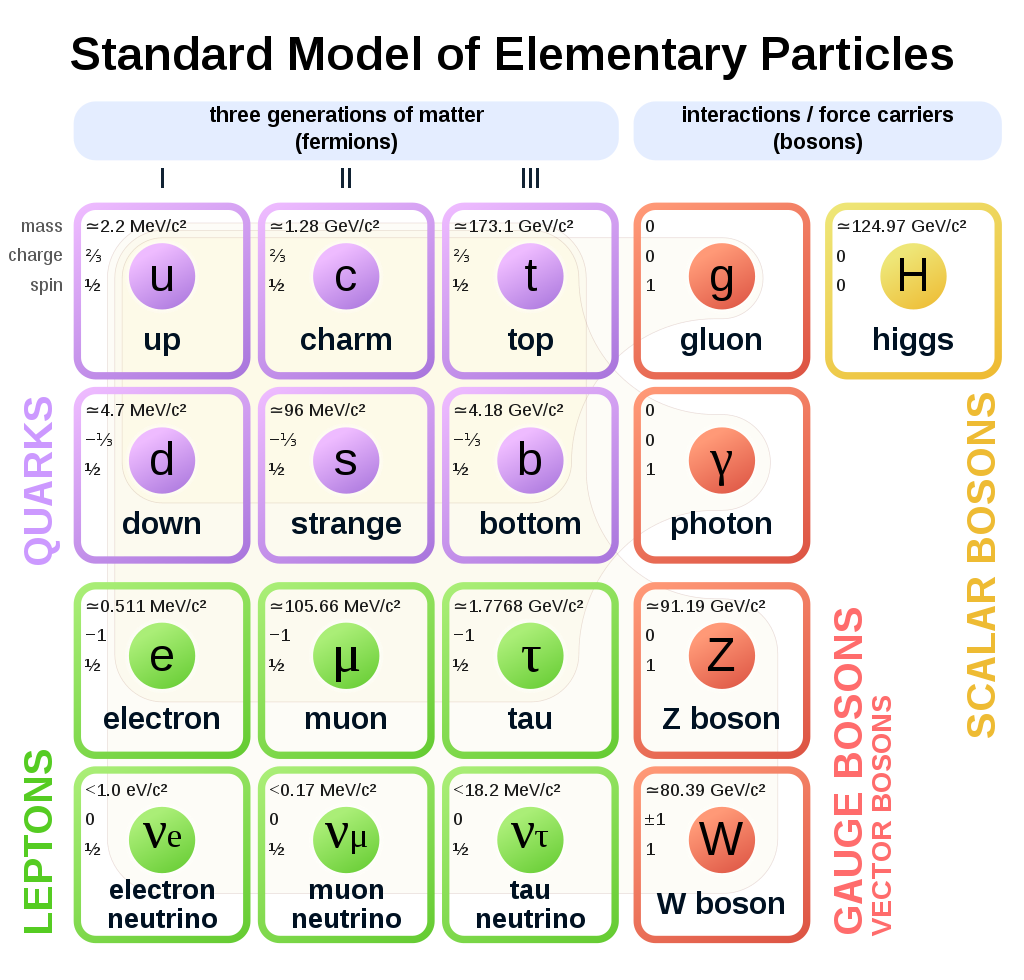
\includegraphics[width=\linewidth]{figures/theory_chapter/SM.png}
\caption{The "periodic table" of the Standard Model, depicting the three generations of fermions, the gauge bosons, and the Higgs \cite{WikipediaSM}.}
\end{figure}

\subsection{Lagrangians, Fields, and Gauge Transformations}\label{sec:Lagrangians}

In order to fully explain the Higgs mechanism, we must first discuss the mathematical language of quantum field theory. Both quantum and classical field theories are often discussed using Lagrangian dynamics, where the Lagrangian is defined as  $\mathcal{L} = T - V$, the difference of the kinetic and the potential energy. Physical properties will always evolve in such a way that the integral of this property with respect to time, $\mathcal{S} = \int \mathcal{L} dt$, called the action, is a constant. Lagrangians are also incredibly useful in that they give rise to conservation laws: Noether's Theorem states that operations performed on a system that do not change the Lagrangian are each associated to conserved quantities of a system (i.e., systems with translationally invariant Lagrangians must respect conservation of momentum, systems with temporally-invariant Lagrangians must respect conservation of energy, etc.).

A variety of types of fields exist, but we will discuss three at length: Klein-Gordon fields, which are scalar fields (single quantities defined everywhere), Dirac spinor fields (vector quantities defined everywhere), and gauge fields (additional vector fields that must be introduced in order to preserve certain physical symmetries. We begin with the Klein-Gordon field.

Klein-Gordon fields, one of the simplest examples of a field, are real scalar-valued quantities often denoted using the symbol $\phi$. A non-interacting "free" Klein-Gordon field evolves according to the Lagrangian:

\begin{flalign}
  \begin{aligned}
\mathcal{L} = T - V \\
=\frac{1}{2} \frac{\partial^{2} \phi}{\partial t^{2}} - \frac{1}{2} (\nabla \phi)^{2} - \frac{1}{2} m^{2} \phi^{2} \\
=-\frac{1}{2}(\partial^{\mu}\phi)(\partial_{\mu}\phi)- \frac{1}{2} m^{2} \phi^{2}
  \end{aligned}&&&
\end{flalign}

where we utilize Einstein sum notation in the last line to compress the four derivatives in the preceding expression into a single shorthand symbol. The Lagrangian of an interacting Klein-Gordon field would look similar, but would possess additional $V$ potential terms depending on the nature of the interaction. As the only scalar in the Standard Model, the observable Higgs boson is the only elementary particle to follow an interacting Klein-Gordon field equation.

While the concept of a complex-valued scalar field does not directly correspond to any of the physical elementary particles that are present in the Standard Model, it plays an important role in the understanding of the Higgs mechanism. A complex-valued scalar field behaves similarly to a real-valued one, with the Lagrangian:

\begin{equation}
\mathcal{L} = (\partial^{\mu}\phi^{*})(\partial_{\mu}\phi) - \frac{1}{2} m^{2} \phi^{*} \phi
\end{equation}

Where * denotes the complex conjugate of the scalar field.

Finally, Dirac fields describe all Standard Model fermions (with the possible exception of neutrinos). They are vector fields as opposed to scalar fields, and behave according to the Lagrangian:

\begin{equation}
\mathcal{L} = \bar{\psi}(i \gamma^{\mu} \partial_{\mu} - m) \psi
\end{equation}

where $\gamma^{\mu}$ denotes the set of Dirac gamma matrices, and $\bar{\psi} = \psi^{\dag} \gamma^0$ denotes the transpose of the complex conjugate of the vector field multiplied by one of these matrices, defined as such in order to preserve invariance under relativistic Lorentz boosts. 

A four-component Dirac vector field can be written in a variety of representations, but one of the most useful is that of a doublet of two two-component Weyl spinors, one left-handed and one right-handed, that is, $\psi = \begin{pmatrix} \psi_L \\ \psi_R \end{pmatrix}$. Each of these components transforms differently under Lorentz boosts.

In order to discuss the gauge fields corresponding to the Standard Model bosons, we must first discuss the concept of gauge symmetries. Consider a single Dirac vector field described by equation \ref{eq:Dirac}. We transform the field by rotating it by a constant phase $\alpha$:  $\psi \rightarrow e^{i \alpha} \psi $, $\bar{\psi} \rightarrow e^{-i \alpha} \bar{\psi} $.

\begin{flalign}
  \begin{aligned}
\mathcal{L} = - (e^{-i \alpha} \bar{\psi})(i \gamma^{\mu} \partial_{\mu} - m) (e^{i \alpha} \psi) \\
= - (e^{-i \alpha} e^{i \alpha})\bar{\psi} (i \gamma^{\mu} \partial_{\mu} - m)\psi \\
= -\bar{\psi}(i \gamma^{\mu} \partial_{\mu} - m) \psi 
  \end{aligned}&&&
\end{flalign}

We see that we recover the original Dirac Lagrangian. Thus, the lagrangian is invariant under a constant phase rotation. A transformation of this charater is called a global gauge transformation. A one-dimensional rotation is a unitary transformation, so we call this a global $U(1)$ gauge symmetry.

We next consider the concept of a local gauge transformation, that is, one in which the phase $\alpha$ may vary with position. The field transforms, as before, like  $\psi \rightarrow e^{i \alpha (x)} \psi $, $\bar{\psi} \rightarrow e^{-i \alpha (x)} \bar{\psi} $. However, we note that the dependence on position means that we can no longer factor out the exponentials, and we thus have

\begin{flalign}
  \begin{aligned}
\mathcal{L} = - (e^{-i \alpha (x)} \bar{\psi})(i \gamma^{\mu} \partial_{\mu} - m) (e^{i \alpha (x)} \psi) \\
=-i e^{-i \alpha (x)} \bar{\psi} \gamma^{\mu} (e^{i \alpha (x)} \partial_{\mu} \psi  + i e^{i \alpha (x)} \psi \partial_{\mu} \alpha -m \bar{\psi}\psi \\
=-\bar{\psi}(i \gamma^{\mu} \partial_{\mu} + \gamma^{\mu} \partial_{\mu} \alpha - m) \psi
  \end{aligned}&&&
\end{flalign}

i.e., the Lagrangian is not invariant under this sort of transformation. However, local gauge invariance is an important physical symmetry, so in order to attempt to preserve it, we add an additional term to the original Lagrangian: an extra vector field $A_\mu$ that transforms like $A_\mu \rightarrow A_\mu - \frac{1}{q} \partial_{\mu} \alpha(x) $ for a constant q. We also define a new operator, called the covariant derivative: $D_{\mu} = \partial_{\mu}+ iqA_{\mu} $. Given how $A_{\mu}$ transforms, we see that $D_{\mu}$ transforms like

\begin{flalign}
  \begin{aligned}
D_{\mu} = \partial_\mu + iqA_{\mu} \\
\rightarrow \partial_\mu + iq(A_{\mu}-\frac{1}{q}\partial_{\mu}\alpha(x)) \\
= \partial_\mu + iqA_{\mu}-i\partial_{\mu}\alpha(x) \\
=D_{\mu}-i\partial_{\mu}\alpha(x)
  \end{aligned}&&&
\end{flalign}

Let us replace the $\partial_{\mu}\phi$ terms in the initial Lagrangian with $D_{\mu}\phi$ and transform.

\begin{flalign}
  \begin{aligned}
\mathcal{L} = - (e^{-i \alpha (x)} \bar{\psi})(i \gamma^{\mu} (D_{\mu}-i\partial_{\mu}\alpha(x)) - m) (e^{i \alpha (x)} \psi) \\
=-(e^{-i \alpha (x)} \bar{\psi})(i \gamma^{\mu} (\partial_\mu + iqA_{\mu}-i\partial_{\mu}\alpha(x))-m)(e^{i \alpha (x)} \psi) \\
=-\bar{\psi}(i \gamma^{\mu} D_{\mu} + \gamma^{\mu} \partial_{\mu} \alpha - \gamma^{\mu} \partial_{\mu} \alpha - m) \psi \\
=-\bar{\psi}(i \gamma^{\mu} D_{\mu} - m) \psi
  \end{aligned}&&&
\end{flalign}

Thus, by introducing an additional vector field that corresponds to the local U(1) gauge symmetry, we have restored the invariance of our lagrangian. Physically, this field is analogous to the introduction of electromagnetism to our single Dirac fermion model, with the $A_\mu$ field playing the role of the photon: it is a vector quantity and so has spin-1, it must be massless (as adding an $A_\mu$ mass term to the Lagrangian would violate the symmetry again), and couples to the fermion fields according to their electromagnetic charge. We note that we can also still preserve invariance if we add an additional term $L_{kin} = -\frac{1}{4}F^{\mu \nu} F_{\mu \nu}$ to the Lagrangian, where $F_{\mu \nu} = \partial_{\mu} A_{\nu} - \partial_{\nu} A_{\mu}$: this corresponds to the energy inherent in electromagnetic fields themselves. 

Each of the fundamental forces in the Standard Model can be understood in terms of these sorts of gauge symmetries. The photon is the particle excitiation of the electromagnetic field, which corresponds to a one-dimensional rotation "U(1)" transformation. In order to be invariant under three dimensional transformations of the type "SU(3)" (the set of all volume-preserving, $\bar{\psi}\psi$-preserving transformations in a 3D vector space), we must add eight new vector fields (these are the eight gluons), leading to the incorporation of the strong interaction into the Standard Model.

Similarly, in order to be invariant under two-dimensional transformations of the type "SU(2)" (the set of all volume-preserving, $\bar{\psi}\psi$-preserving transformations in a 2D vector space), we must add three new vector fields. However, these cannot be the observed weak-interaction bosons, the $W^{+}, W^{-} and Z$: as mentioned before, the new fields must be massless, as adding a mass term for these bosons would violate the local gauge symmetry. How, then, can the masses of the weak bosons fit into the Standard Model? The answer lies in the introduction of yet another field, called the Higgs field, the particle excitation of which is the much-lauded Higgs boson.

\section{CP-Symmetry}\label{sec:CPT}

In addition to the $SU(2)_{L} \times U(1) \times SU(3)$ gauge symmetry, the Standard Model also respects a discrete symmetry called CPT. This is the combined product of three separate symmetries: charge conjugation (C), parity inversion (P), and time reversal (T). While some interactions may respect a limited combination of these symmetries (i.e., just C, or the product CP), all Standard Model processes must respect the product of the three: that is, for a given physics process, if we invert all the charges, flip all the parities, and run the interaction backward, the resulting new process must also be physically allowed.

The strong nuclear, electromagnetic, and gravitational interactions are symmetric under C, P, and T individually. The weak nuclear interaction, however, is invariant only under the combination of all three: it violates C, P, and, in some cases, CP. The CP violation that occurs in the weak interaction is through the CKM off-diagonal quark-mixing matrix mentioned briefly in section \ref{sec:SM}.

A parity inversion is equivalent to reversing a particle's momentum without reversing its spin. For a fermion field $\psi(t,x)$, a parity transform P takes $\psi(t,x)$ to $\psi(t,-x)$, and looks like $P \psi(t,x) P = e^{i \theta} \gamma^{0} \psi(t,-x)$ for some constant matrix $\theta$. 

Given this, we find that the expression $P \bar{\psi}\psi P = \bar{\psi}\psi$ , so $\bar{\psi}\psi$ is a $\emph{scalar}$ under parity, while the expression $iP \bar{\psi}\gamma^{5}\psi P = -i\bar{\psi}\gamma^{5}\psi$ acquires a minus sign, so $i\bar{\psi}\gamma^{5}\psi$ is a $\emph{pseudoscalar}$ under parity.

A time-reversal is equivalent to "running a process backward". For example, a swinging pendulum is a process that is approximately T symmetric, as it looks similar "played" in forward or reverse, while a plate shattering on the ground is not a T symmetric process, as reversing it does not make physical sense (broken plates do not spontaneously reform). For a fermion field $\psi(t,x)$, a time-reversal transform T takes $\psi(t,x)$ to $\psi(-t,x)$, and looks like $T \psi(t,x) T = -\gamma^{1}\gamma^{3} \psi(-t,x)$. Given this, we find that the expression $T \bar{\psi}\psi T = \bar{\psi}\psi$ , so $\bar{\psi}\psi$ is a $\emph{scalar}$ under parity, while the expression $iT \bar{\psi}\gamma^{5}\psi T = -i\bar{\psi}\gamma^{5}\psi$ acquires a minus sign, so $i\bar{\psi}\gamma^{5}\psi$ is a pseudoscalar under time-reversal.

A charge conjugation is a reversal of all charges (electric charge, weak hypercharge, and strong-nuclear color charge). For a fermion field $\psi(t,x)$, a charge conjugation transform C takes $\psi$ to $\bar{psi}$, and looks like $C \psi C = -i (\bar{\psi} \gamma^{0} \gamma^{2})^{T}$ (where T here denotes the matrix transpose). Given this, we find that the expression $C \bar{\psi}\psi C = \bar{\psi}\psi$ , so $\bar{\psi}\psi$ is a $\emph{scalar}$ under charge conjugtion, as is the expression $iC \bar{\psi}\gamma^{5}\psi C = i\bar{\psi}\gamma^{5}\psi$ is as well. Thus, Lagrangians containing terms of the form $i\bar{\psi}\gamma^{5}\psi$ are invariant under C and CPT, but not P, T or CP.

Applying C and P together is equivalent to switching particles and antiparticles. However, we also know that our universe is composed almost entirely of matter, and not equal parts matter and antimatter (living in a universe in which matter and antimatter are equally abundant would be very unpleasant, as the two would be constantly annhilating each other, bathing us in a near-constant shower of gamma rays) \cite{Sakharov}. Thus, some physics process that occurs in the high-energy regime near the Big Bang must violate CP in a substantial way. The CP-invariance that occurs through the CKM mixing is not enough to account for the matter-antimatter asymmetry, so searching for this source of CP violation is of pressing interest to experimental physicists \cite{CKM}.

\section{The Higgs Mechanism and Electroweak Symmetry Breaking} \label{sec:EWSB} 

Given the results of previous sections, it should be clear that the Higgs field is important not simply because it "gives particles mass" (an often-made claim which is, in a sense, true), but because it is a vital missing piece of the Standard Model that is necessary to reconcile the elegant mathematical language of the fundamental interactions with the particles we observe in real-world experiments \cite{Higgs}.

To understand the Higgs mechanism, we must first devote a brief detour to the concept of spontaneous symmetry breaking. This occurs when an unstable, continuous symmetric state spontaneously changes into a more stable, asymmetric one. Consider, for example, the "wine-bottle" potential shape depicted in figure \ref{fig:potential}.

\begin{figure}
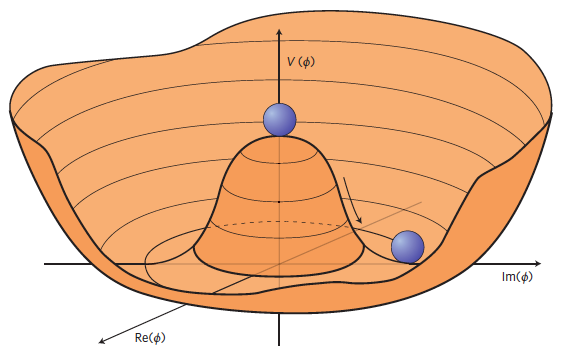
\includegraphics[width=\linewidth]{figures/theory_chapter/higgspotential.png}
\caption{The "wine bottle" Higgs potential hill, from reference \cite{EllisHiggs}}
\label{fig:potential}
\end{figure}

When the ball is balanced at the top of the potential "hill", the configuration is spatially symmetric: that is, no direction is privileged over any other. However, when this delicate balance is even slightly disturbed, the ball will roll down the hill in some direction, resulting in a final state that is $\emph{not}$ symmetrical. This is the phenomenon known as "spontaneous symmetry breaking".

Using the language of quantum field theory, we can easily add spontaneously-breakable symmetric potential terms to a Lagrangian. If we do so, the phenomenon of symmetry breaking allows us to rewrite these terms as a combination of massless fields (one for each "choice" the symmetry breaking must make) and massive fields (corresponding to the leftover degrees of freedom). If we rewrite the "wine-bottle" potential in this way, for example, the one new massless field corresponds to the ball's angular position along the circle at the base, while the massive field corresponds to the ball's  radial position "up" or "down" the hill. The massless particles that arise from these massless fields are known as Goldstone bosons.

We are now ready to discuss the Higgs mechanism. We can combine the electromagnetic and weak nuclear forces as different manifestations of the same force, called the electroweak force, that transforms like $U(1) \times SU(2)$. We write the terms of the Standard Model electroweak Lagrangian, noting that, since the weak interaction is observed to be chiral, it couples differently to left- and right-handed fermions.

In this case, the generator of the U(1) symmetry ($\alpha(x)$) is not the electric charge $Q$ as in our previous example, but is instead the "Weak Hypercharge" $Y = 2(Q -I_{3})$, where $I_{3}$ is the third component of the "Weak Isospin" $I$. For right-handed particles, $I_{3} = 0$, for left-handed up/charm/top quarks and neutrinos, $I_{3} = +\frac{1}{2}$, and for left-handed down/strange/bottom quarks and charged leptons, $I_{3} = +\frac{1}{2}$. We will call our U(1) boson $B_{\mu}$ rather than $A_{\mu}$, to distinguish it from the photon. For a fermion $\psi$ (u/c/s/e/$\mu$/$\tau$) that couples weakly to another fermion $\psi'$, we can write the left-and-right-handed components of f as 

$L = \begin{pmatrix} \psi_{L} \\ \psi'_{L} \end{pmatrix}$, $R = \begin{pmatrix}\psi_{R} \end{pmatrix}$.

Similarly, the generators of the SU(2) symmetry are the three matrices $\tau_{i}$, one corresponding to each weak boson $W^{\mu}_{i}$. The self-interaction term for the weak interaction is $L_{kin} = -\frac{1}{4}G^{\mu \nu}G_{\mu \nu}$, where $G_{\mu \nu} = \partial_{\mu} W_{\nu} - \partial_{\nu} W_{\mu}+\frac{g}{2} W_{\mu}\times W_{\nu}$.

We can define a new covariant derivative capturing the weak interaction terms as well: $D^{\mu} = \partial^{\mu}- \frac{1}{2}iYg_{1}B^{\mu} -\frac{1}{2}i I g_2 \Sigma \tau_{i}W_{i}^\mu$ Thus, the full electroweak $SU(2)_L \times U(1)$ Lagrangian is:

\begin{equation}
\mathcal{L} = i\bar{R}\gamma^{\mu}D_{\mu}R + i\bar{L}\gamma^{\mu}D_{\mu}L -\frac{1}{4}G^{\mu \nu}G_{\mu \nu} -\frac{1}{4}F^{\mu \nu} F_{\mu \nu}
\end{equation}

However, we note that this Lagrangian does not allow for gauge boson mass or fermion mass, as a fermion mass term $m\bar{\psi}\psi = m(\bar{\psi_{R}}\psi_{L}+\bar{\psi_{L}}\psi_{R})$ is not an SU(2) singlet and would thus not be invariant under the SU(2) symmetry. 

To rectify this, we can introduce a new complex SU(2) doublet scalar field $\phi = \begin{pmatrix} \phi^{+} \\ \phi^{0} \end{pmatrix} = \begin{pmatrix} \phi_{1} + i\phi_{2}  \\ \phi_{3} + i\phi_{4} \end{pmatrix}$ called the $\emph{Higgs field}$. It follows the Lagrangian

\begin{equation}
\mathcal{L} = T-V = (D^{\mu}\phi)^{\dag}(D_{\mu}\phi) - {\mu}^2\phi^{\dag}\phi - \lambda(\phi^{\dag}\phi)^{2}
\end{equation}

which, if $mu^{2} < 0$ has a minimum at
\begin{equation}
\phi^{\dag}\phi = \frac{-\mu^{2}}{2 \lambda} = \frac{v^{2}}{2}
\end{equation}

We note that the potential is symmetric, so we can pick a direction to "break the symmetry" in. Let us define the vacuum as $\phi_0 = \frac{1}{\sqrt{2}} \begin{pmatrix} 0 \\ v \end{pmatrix}$. Then, for any arbitrary configuration of the field, we can expand the potential about the minimum as $\phi(x) = \frac{1}{\sqrt{2}} \begin{pmatrix} 0 \\ (v + h(x)) \end{pmatrix}$.

We can expand the kinetic term in the Lagrangian as

\begin{equation}
(D^{\mu}\phi)^{\dag}(D_{\mu}\phi) = \frac{1}{2}(\partial_{\mu}h)(\partial^{\mu}h)+ \phi^{\dag}(\frac{1}{2}iYg_{1}B_{\mu} -\frac{1}{2}iI g_2 \Sigma \tau_{i}W_{i\mu})^{\dag}(\frac{1}{2}iYg_{1}B^{\mu} -\frac{1}{2}iI g_2 \Sigma \tau_{i}W_{i}^mu) \phi
\end{equation} 

Which, using the definitions of the three tau matrices, and putting Y = I = 1, becomes

\begin{flalign}
  \begin{aligned}
\frac{1}{2}(\partial_{\mu}h)(\partial^{\mu}h) + \frac{1}{8} |\begin{bmatrix} g_{1}B_{\mu}+g_{2}W_{\mu}^{3} & g_{2}(W_{\mu}^{1}-iW_{\mu}^{2}) \\ g_{2}(W_{\mu}^{1}+iW_{\mu}^{2}) & g_{1}B_{\mu}+g_{2}W_{\mu}^{3} \end{bmatrix} \begin{bmatrix} 0 \\ v \end{bmatrix}|^{2} \\
= \frac{1}{2}(\partial_{\mu}h)(\partial^{\mu}h) + \frac{1}{8}v^{2}g_{2}^{2}((W_{\mu}^{1})^{2}+(W_{\mu}^{2})^{2})) + \frac{1}{8}v^{2}(g_{1} B{\mu}-g_{2}W_{\mu}^{3})^{2}
  \end{aligned}&&&
\end{flalign}

If we again define some new field combinations here: $W_{\mu}^{+} -\frac{1}{\sqrt{2}}(W_{\mu}^{1}-iW_{\mu}^{2})$, $W_{\mu}^{-} -\frac{1}{\sqrt{2}}(W_{\mu}^{1}+iW_{\mu}^{2})$, $Z_{\mu} = \frac{g_{1}B{\mu}+g_{2}W_{\mu}}{\sqrt{{g_1}^2+{g_2}^2}}$ and $A_{\mu} = \frac{g_{1}B{\mu}-g_{2}W_{\mu}}{\sqrt{{g_1}^2+{g_2}^2}}$,

then we get: 
\begin{equation}
\frac{1}{2}(\partial_{\mu}h)(\partial^{\mu}h) + (\frac{1}{2}vg_{2})^{2}W_\mu^{+}W_\mu^{-}+(\frac{1}{2}v(\sqrt{{g_1}^2+{g_2}^2}))^{2}Z_{\mu}
\end{equation}

And we see that Z field and the two W fields have acquired mass terms, while the A field has remained massless. This corresponds to what we observe in the real world: the W bosons and the Z boson are massive, while the photon remains massless!

For fermions, the coupling to the Higgs field looks like $g_{f}(\bar{f}_{L}\phi f_{R} + \phi^{\dag}\bar{f}_{R} f_{L})$ (for some constant $g_{f}$).

We note that, if we expand $\phi(x) = \frac{1}{\sqrt{2}} \begin{pmatrix} 0 \\ (v + h(x)) \end{pmatrix}$ as before, we find that the coupling term now looks like 
$\frac{g_{f}v}{\sqrt{2}}(\bar{f}_{L}f_{R} + \bar{f}_{R}f_{L}) + \frac{g_{f}}{\sqrt{2}}(\bar{f}_{L}f_{R} + \bar{f}_{R}f_{L})$. Thus, the presence of the Higgs field allows us to have fermion mass terms in our Lagrangians, where the masses are $m_{f} = \frac{g_{f}v}{\sqrt{2}}$. However, we note that, at the current time, there is no way to derive the $g_{f}$ coupling theoretically: thus, while the Higgs mechanism now allows us to have massive fermions in our theory, it does not actually determine what the masses of these fermions are.

Finally, we note that if we expand the potential term in the complex Klein-Gordon Lagrangian for the Higgs field about the minimum, that is, 

\begin{flalign}
  \begin{aligned}
V = {\mu}^2\phi^{\dag}\phi + \lambda(\phi^{\dag}\phi)^{2} = \frac{1}{2}{\mu}^2(v+h)^{2} + \frac{1}{4}\lambda(v+h)^{4} \\
= -\frac{1}{2}{\lambda v^{2}}(v+h)^{2} + \frac{1}{4}\lambda(v+h)^{4} \\
= -\frac{1}{2}\lambda(v^{4} + 2v^{3}h + v^{2}h^{2}) + \frac{1}{4}\lambda(v^{4}+4vh^{3}+6v^{2}h^{2} + 4v^{3}h + h^{4})
  \end{aligned}&&&
\end{flalign}

we see a mass term of the form $(\frac{M_{h}^{2}}{2})h^{2} = \frac{6}{4}\lambda v^{2} h^{2} - \frac{1}{2}\lambda v^{2} h^{2} = \lambda v^{2} h^{2}$;
That is, $M_{h} = v \sqrt{2 \lambda}$.

In sum: without a Higgs field, in order for the Standard Model electroweak Lagrangian to preserve $SU(2)_L \times U(1)$ symmetry, we are forbidden from including mass terms for the fermions or the gauge bosons. However, by adding this additional field to the model and breaking its symmetry, we find that we can include fermion mass terms that do not violate the $SU(2)_L \times U(1)$ symmetry, and that the electroweak gauge bosons now acquire mass terms by default. Furthermore, this new field also has a mass. This is a remarkable result: by simply adding one extra field to the model, we have solved several different problems in one fell swoop!

\section{The Higgs Boson and Its Couplings} \label{sec:Higgs Couplings} 

As we have seen, the Standard Model Higgs is massive, and couples directly to all other massive particles (with the possible exception of neutrinos; this is an active area of research). However, the existence of the Higgs is clearly not all there is to the story: the Standard Model is noticeably incomplete (What are dark matter and dark energy? What determines the exact masses of each of the fermions? Why have we never observed right-handed neutrinos? Can we unify other forces like we have unified electromagnetism and the weak force?). In the majority of proposed Beyond-the-Standard Model extensions, other particles that would interact with the Standard Model Higgs are introduced, including additional Higgs fields, as well as new massive fermions and bosons.

With the discovery of the Higgs, it can be argued that we have now entered an era of precision-measurement in collider physics. By closely studying interactions that are very sensitive to the injection of new physics, we can potentially detect deviations from the Standard Model: in many cases, we may see hints of the existence of new particles through changes to quantities of interest well before we are actually able to produce these particles in colliders directly. Due to the Higgs coupling to all massive particles, Higgs interactions are especially sensitive to new physics, and thus can serve as a useful bellwether for physics beyond the standard model.

The Large Hadron Collider is a proton-proton collider; as such, physics processes that occur in it are almost always initiated by quarks or gluons. The predominant production modes are, in order of frequency, gluon-gluon fusion ($ggF$), vector boson fusion ($VBF$), vector-boson associated ($VH$) and top-associated ($ttH$). The top-associated Higgs production mode is of particular interest to many experimentalists due to its direct dependence on the Higgs coupling to a fermion- by closely measuring the frequency and properties of the $ttH$ mode, we can better understand the nature of this variety of couplings. Rarer production modes, such as single-top associated Higgs production ($tH$), can shed still more light on the nature of the top-quark/Higgs coupling (called the top quark Yukawa coupling), but are much more difficult to observe. The $tH$ process occurs in two final-state modes, $tWH$ and $tHj$; however, there is some nuance in their definitions which we will come to shortly.

\begin{figure}[htp]
  \centering
         \begin{subfigure}[b]{0.3\textwidth}
         \centering
         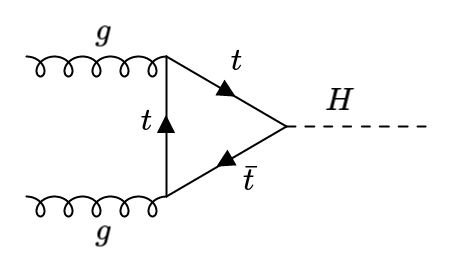
\includegraphics[width=\textwidth]{figures/theory_chapter/ggF.png}
         \caption{ggF}
         \label{fig:ggF}
     \end{subfigure}
     \hfill
       \begin{subfigure}[b]{0.3\textwidth}
         \centering
         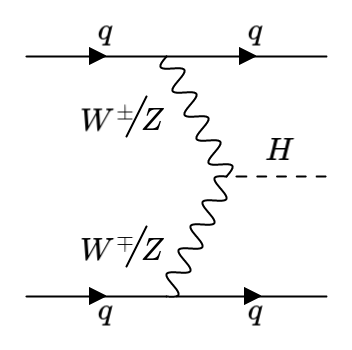
\includegraphics[width=\textwidth]{figures/theory_chapter/VBF.png}
         \caption{VBF}
         \label{fig:VBF}
     \end{subfigure}
     \hfill 
     \\
        \begin{subfigure}[b]{0.3\textwidth}
         \centering
         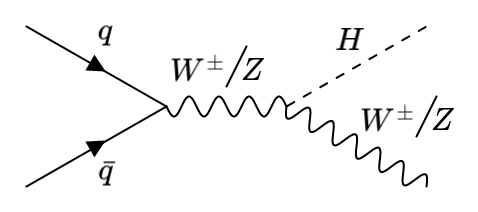
\includegraphics[width=\textwidth]{figures/theory_chapter/VH.png}
         \caption{VH}
         \label{fig:VH}
     \end{subfigure}
  \label{fig:Higgsmodes}
  \caption{Feynman diagrams depicting the three leading Higgs production modes. Made with \cite{FeynmanMaker}}  
\end{figure}

\begin{figure}[htp]
  \centering
       \begin{subfigure}[b]{0.3\textwidth}
         \centering
         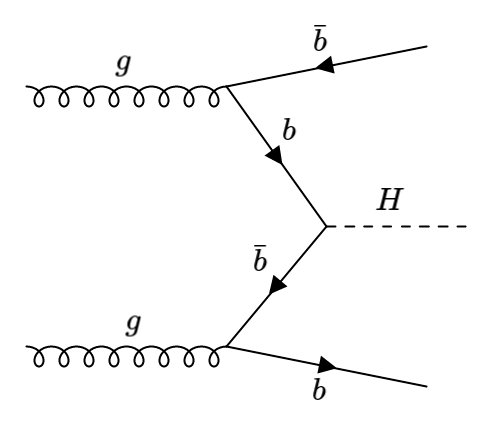
\includegraphics[width=\textwidth]{figures/theory_chapter/bbH.png}
         \caption{bbH}
         \label{fig:bbH}
     \end{subfigure}
     \hfill
         \begin{subfigure}[b]{0.3\textwidth}
         \centering
         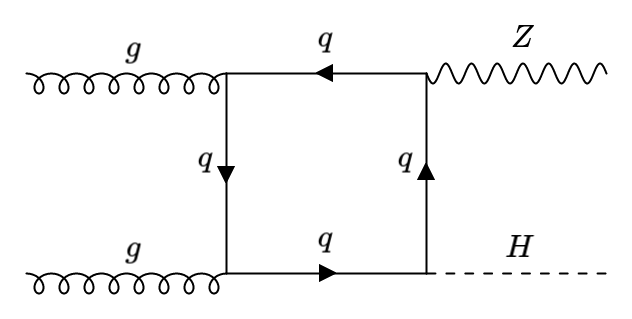
\includegraphics[width=\textwidth]{figures/theory_chapter/ggZH.png}
         \caption{gg $\rightarrow ZH$ }
         \label{fig:ggZH}
     \end{subfigure}
     \hfill
         \begin{subfigure}[b]{0.3\textwidth}
         \centering
         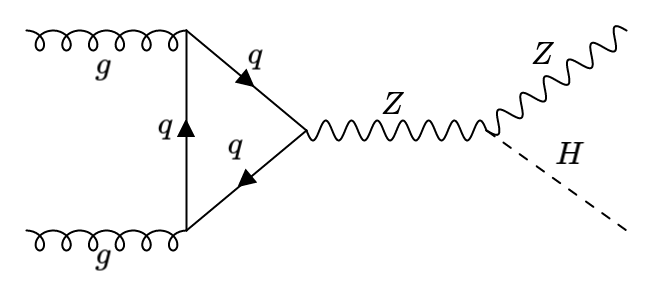
\includegraphics[width=\textwidth]{figures/theory_chapter/ggZH2.png}
         \caption{Additional gg $\rightarrow ZH$ }
         \label{fig:ggZH}
     \end{subfigure}
     \hfill
  \label{fig:loopmodes}
  \caption{Feynman diagrams depicting relevant less-common Higgs production modes.Made with \cite{FeynmanMaker}}  
\end{figure}

\begin{figure}[htp]
  \centering
       \begin{subfigure}[b]{0.3\textwidth}
         \centering
         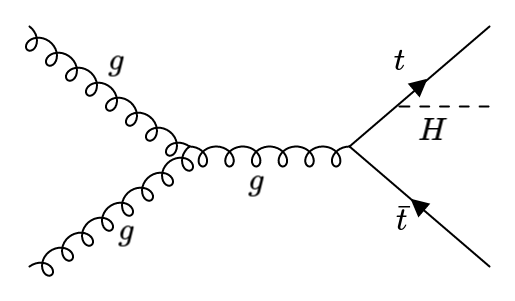
\includegraphics[width=\textwidth]{figures/theory_chapter/ttH1.png}
         \label{fig:ttH1}
     \end{subfigure}
     \hfill
       \begin{subfigure}[b]{0.3\textwidth}
         \centering
         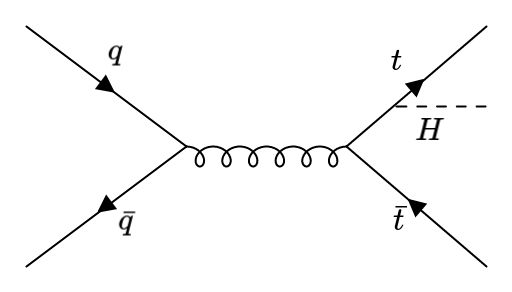
\includegraphics[width=\textwidth]{figures/theory_chapter/ttH2.png}
         \label{fig:ttH2}
     \end{subfigure}
     \hfill
       \begin{subfigure}[b]{0.3\textwidth}
         \centering
         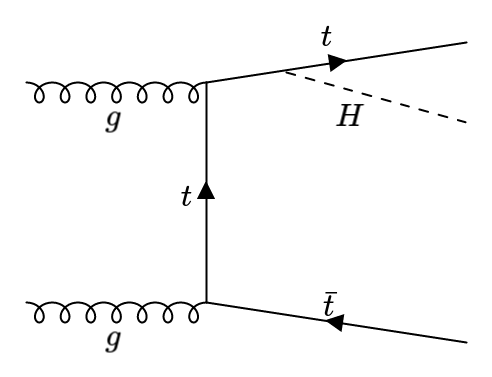
\includegraphics[width=\textwidth]{figures/theory_chapter/ttH3.png}
         \label{fig:ttH3}
     \end{subfigure}
     \hfill
         \begin{subfigure}[b]{0.3\textwidth}
         \centering
         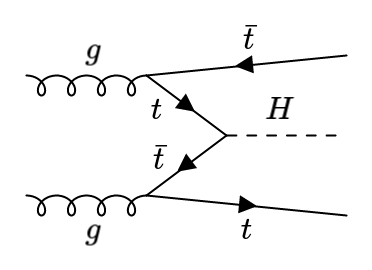
\includegraphics[width=\textwidth]{figures/theory_chapter/ttH4.png}
         \label{fig:ttH4}
     \end{subfigure}
     \hfill 
  \label{fig:loopmodes}
  \caption{Feynman diagrams depicting ttH production modes.Made with \cite{FeynmanMaker}}  
\end{figure}

\begin{figure}[htp]
  \centering
       \begin{subfigure}[b]{0.3\textwidth}
         \centering
         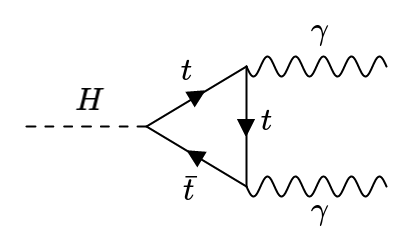
\includegraphics[width=\textwidth]{figures/theory_chapter/toploop.png}
         \caption{Top-mediated}
         \label{fig:toploop}
     \end{subfigure}
     \hfill
         \begin{subfigure}[b]{0.3\textwidth}
         \centering
         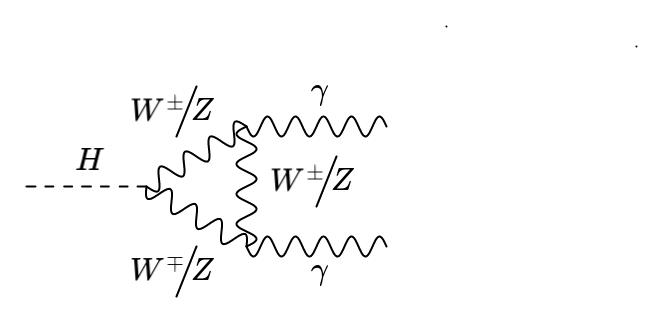
\includegraphics[width=\textwidth]{figures/theory_chapter/Wloop1.png}
         \caption{W $\rightarrow \gamma$ }
         \label{fig:Wloop1}
     \end{subfigure}
     \hfill 
        \begin{subfigure}[b]{0.3\textwidth}
         \centering
         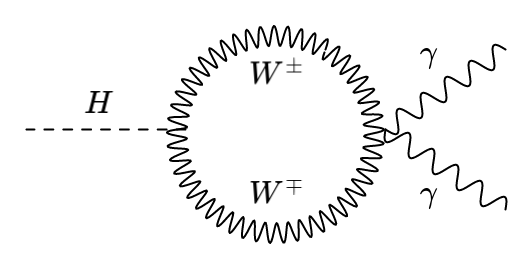
\includegraphics[width=\textwidth]{figures/theory_chapter/Wloop2.png}
         \caption{W $\rightarrow \gamma \gamma$}
         \label{fig:Wloop2}
     \end{subfigure}
     \hfill
  \label{fig:loopmodes}
  \caption{Feynman diagrams depicting the leading-order processes contributing to the Higgs diphoton decay. Made with \cite{FeynmanMaker}}  
\end{figure}

Similarly, the dominant decay mode of the Higgs is to bottom quarks ($H \rightarrow bb$), followed by to W bosons ($H \rightarrow WW$), gluons ($H \rightarrow WW$), tau leptons ($H \rightarrow \tau \tau$), charm quarks ($H \rightarrow bb$), Z bosons ($H \rightarrow ZZ$), photons ($H \rightarrow \gamma \gamma$), and a Z boson and a photon ($H \rightarrow Z \gamma$). Because the Higgs does not couple to massless particles directly, the decays to gg and $\gamma \gamma$ are mediated by loop diagrams, most often involving top quarks.

Investigating each of these decay modes has different benefits and detriments. While the Higgs decay to bottom quarks is the most common, correctly identifying and accurately reconstructing quarks and gluons using the jets that they produce in detectors is often very difficult. Decays to W bosons, Z bosons, and $\tau$ leptons provide "cleaner" channels, but because the W, Z and $\tau$ decay dominantly to hadrons, similar reconstruction issues occur unless we restrict ourselves to the rarer leptonic subchannels of these decays. The Higgs to diphoton channel occurs very rarely, but offers a much more unambiguous signal, as the odds of misidentifying high-energy gamma rays are fairly low.

Additionally, we must consider combinatorics: in the ttH production mode, for instance, the final state contains two bottom quarks from the decay of the associated top quarks. If we choose to examine the subchannel in which the Higgs decays to bottom quarks as well, we find that we have at least four final-state bottom quark jets in the event, with 12 different unique assignments of bottom quark jets to parent particles. Correctly matching up which jet originated from which parent particle thus further complicates the reconstruction problem.

The rate of a particular physics production mode or scattering process is parameterized using a quantity called the cross-section $\sigma$, which is measured in units of "barns". Similarly, the rate of a particular decay process is parameterized using a quantity called the decay width $\Gamma$, which measures the probability of a particular decay occurring per unit time. We can also define the "Branching Fraction" of a particular process: if $\Gamma_{H}$ denotes the sum of all Higgs decay widths, for a given process $H \rightarrow XX$ we define

\begin{equation}
Br(H \rightarrow XX) = \frac{\Gamma(H \rightarrow XX)}{\Gamma_{H}}
\end{equation}

\begin{figure}
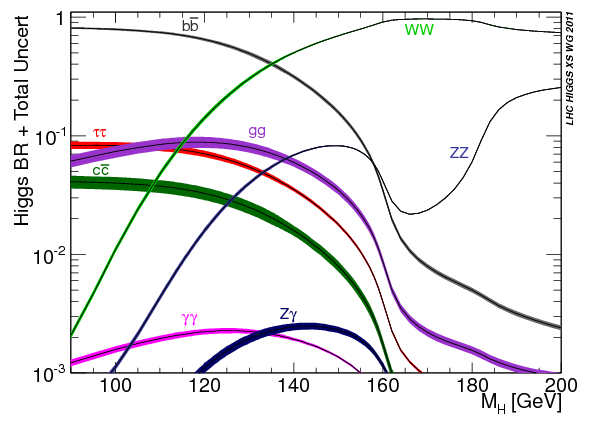
\includegraphics[width=\linewidth]{figures/theory_chapter/HiggsBR.png}
\caption{The branching ratio of the Higgs to various final state particles as a function of its mass (now known to be ~125 GeV), from reference \cite{YellowReport1}.}
\end{figure}

\begin{table}[h]
    \centering
    \begin{tabular}{cc}
        	Decay Mode & Branching fraction [\%] \\
            $H \rightarrow bb $ & $ 57.5 \pm 1.9 $ \\
			$H \rightarrow WW $ & $ 21.6 \pm 0.9 $ \\
			$H \rightarrow gg $ & $ 8.56 \pm 0.86 $ \\
			$H \rightarrow \tau \tau $ & $ 6.30 \pm 0.36 $ \\
			$H \rightarrow cc $ & $ 2.90 \pm 0.35 $ \\
			$H \rightarrow ZZ $ & $ 2.67 \pm 0.11 $ \\
			$H \rightarrow \gamma \gamma $ & $ 0.228 \pm 0.011 $ \\
			$H \rightarrow Z \gamma $ & $ 0.155 \pm 0.014 $ \\
			$H \rightarrow \mu \mu $ & $ 0.022 \pm 0.001 $ \\
    \end{tabular}
    \caption{Higgs decay modes and branching fractions, for a Standard Model Higgs with mass of 125.09 GeV \cite{YellowReport4}}
    \label{mytable}
\end{table}

Cross-sections are calculated at a given perturbation-theoretic "order", indicating how many additional correction terms (often indicated by Feynman diagrams with internal loops and vertices) are accounted for in the calculation- for a given process, leading-order (or "LO"), next-to-leading order ("NLO"), and next-to-next-to-leading order ("NNLO") indicate increasing numbers of correction terms. Calculating and simulating to higher orders is more accurate, but is often much more computationally expensive. These correction terms can be applied for both electroweak (EW) and quantum-chromodynamical (QCD) effects.

In addition to considering which corrections to apply, we must also consider the flavor scheme of the Monte Carlo generator. Physics processes can be initiated by real quarks or gluons that are present in the initial scattering protons, as well as virtual quarks that are present in the primordial soup of energy that binds each proton together. In the five-flavor Parton Distribution Function (PDF) scheme, we consider massless virtual bottom quarks to be constituents of the proton that are capable of initiating physics processes, while in the four-flavor PDF scheme, we do not. These schemes differ primarily in which diagrams they treat as corrections and which they do not- thus, if we perform QCD corrections at all orders (that is, NN...NNLO), we find that these two schemes produce identical results \cite{FedericotH}. Diagrams from the five-flavor PDF scheme that are initiated by a bottom quark can be mapped into the four-flavor scheme by adding an additional bottom-quark to the final state; however, for $ttH$, $tt\gamma\gamma$ and $tWH$ processes, this presents a number of nontrivial modelling issues \cite{FedericotWH}. While the five-flavor scheme offers easier calculation and the ability to model more processes, the four-flavor scheme is better at modelling Higgs kinematics, such as $p_{T}$ and bottom-quark  $p_{T}$. For these reasons, we use the four-flavor scheme to model the $tHj$ process only (henceforth called $tHjb$ due to the presence of the additional final-state b-jet) and the five-flavor scheme for all other top-quark-based processes. 

\begin{figure}[htp]
  \centering
       \begin{subfigure}[b]{0.3\textwidth}
         \centering
         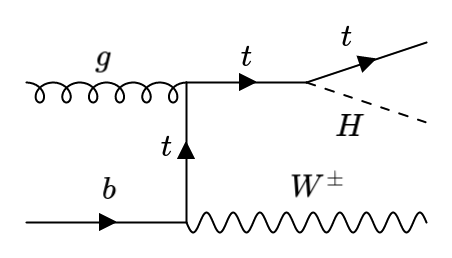
\includegraphics[width=\textwidth]{figures/theory_chapter/tWH1.png}
         \caption{A tWH mode}
         \label{fig:tWH1}
     \end{subfigure}
     \hfill
         \begin{subfigure}[b]{0.3\textwidth}
         \centering
         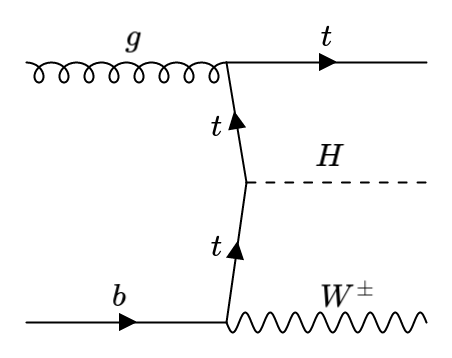
\includegraphics[width=\textwidth]{figures/theory_chapter/tWH2.png}
         \caption{A tWH mode}
         \label{fig:tWH2}
     \end{subfigure}
     \hfill
         \begin{subfigure}[b]{0.3\textwidth}
         \centering
         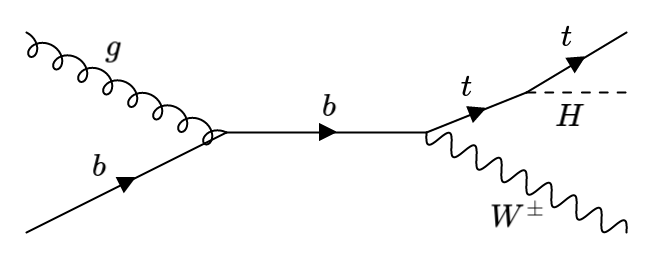
\includegraphics[width=\textwidth]{figures/theory_chapter/tWH3.png}
         \caption{A tWH mode}
         \label{fig:tWH3}
     \end{subfigure}
     \hfill
         \begin{subfigure}[b]{0.3\textwidth}
         \centering
         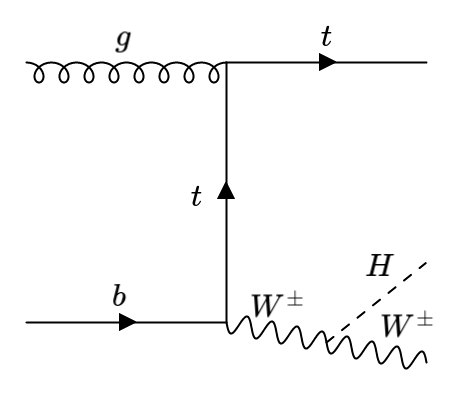
\includegraphics[width=\textwidth]{figures/theory_chapter/tWH4.png}
         \caption{A tWH mode}
         \label{fig:tWH4}
     \end{subfigure}
     \hfill
         \begin{subfigure}[b]{0.3\textwidth}
         \centering
         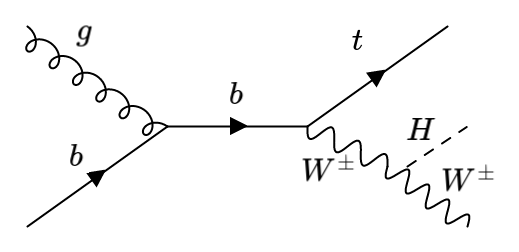
\includegraphics[width=\textwidth]{figures/theory_chapter/tWH5.png}
         \caption{A tWH mode}
         \label{fig:tWH5}
     \end{subfigure}
  \label{fig:tWHmodes}
  \caption{Feynman diagrams depicting the leading-order terms for $tWH$. Because all diagrams contain initial b-quarks, all of these processes can only occur in the five-flavor PDF scheme. Made with \cite{FeynmanMaker}}  
\end{figure}

\begin{figure}[htp]
  \centering
       \begin{subfigure}[b]{0.3\textwidth}
         \centering
         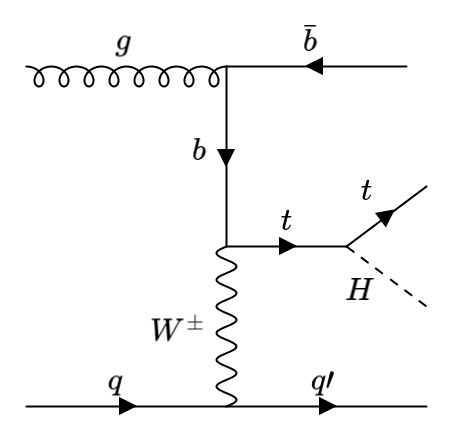
\includegraphics[width=\textwidth]{figures/theory_chapter/tHjb1.png}
         \caption{A tHjb mode}
         \label{fig:tHjb1}
     \end{subfigure}
     \hfill
         \begin{subfigure}[b]{0.3\textwidth}
         \centering
         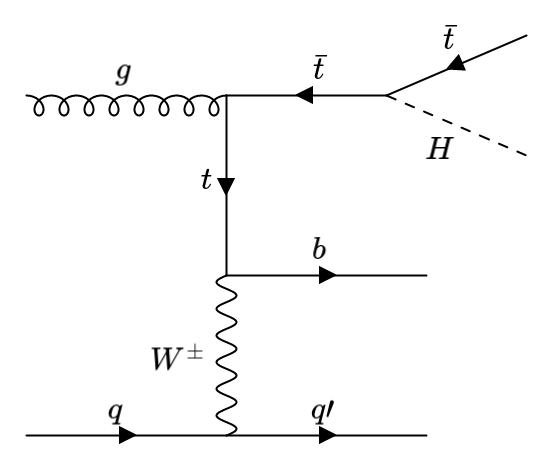
\includegraphics[width=\textwidth]{figures/theory_chapter/tHjb2.png}
         \caption{A tHjb mode}
         \label{fig:tHjb2}
     \end{subfigure}
     \hfill
         \begin{subfigure}[b]{0.3\textwidth}
         \centering
         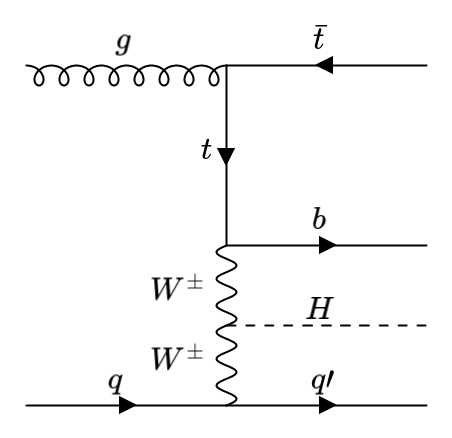
\includegraphics[width=\textwidth]{figures/theory_chapter/tHjb3.png}
         \caption{A tHjb mode}
         \label{fig:tHjb3}
     \end{subfigure}
     \hfill
         \begin{subfigure}[b]{0.3\textwidth}
         \centering
         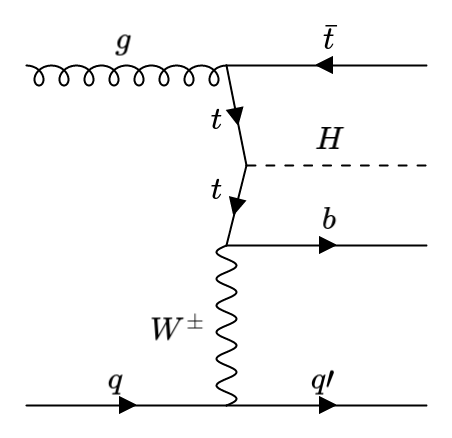
\includegraphics[width=\textwidth]{figures/theory_chapter/tHjb4.png}
         \caption{A tHjb mode}
         \label{fig:tHjb4}
     \end{subfigure}
     \hfill
         \begin{subfigure}[b]{0.3\textwidth}
         \centering
         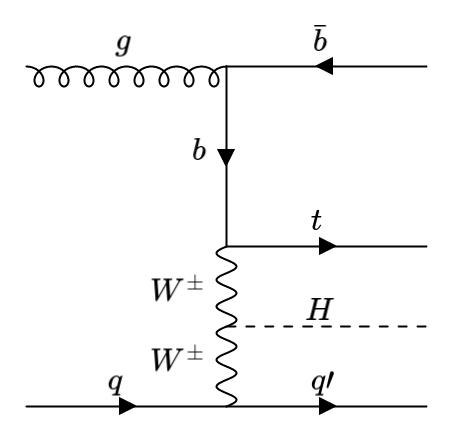
\includegraphics[width=\textwidth]{figures/theory_chapter/tHjb5.png}
         \caption{A tHjb mode}
         \label{fig:tHjb5}
     \end{subfigure}
  \label{fig:tHjbmodes}
  \caption{Feynman diagrams depicting the leading-order terms for $tHjb$, made with \cite{FeynmanMaker}. These diagrams are calculated using the four-flavor PDF scheme. Note that additional diagrams can be created by reversing the direction of the upper fermion "circuit" (the final-state top and bottom must be opposite sign, but $tHj\bar{b}$ and $\bar{t}Hjb$ are equally likely to occur).}  
\end{figure}

\subsection{The Kappa Framework} \label{sec:kappaFW}

This dissertation features two physics analyses from the ATLAS experiment. The first is a targeted attempt to measure whether the top quark Yukawa coupling is CP-even (respects CP symmetry) or CP-odd (violates it) by closely studying the $ttH$ process. In the Standard Model Lagrangian, the top Yukawa coupling is purely CP-even, and can be written in the form $\kappa g_{t} \bar{t}th$. Adding a CP-odd component to the coupling adds an additional $\kappa g_{t} \bar{t} (i \gamma^{5})th$ term to the Lagrangian; the total coupling can thus be parameterized as $\kappa g_{t} \bar{t} (cos(\alpha)+ sin(\alpha) i \gamma^{5} )th$ for a "CP-mixing angle" $\alpha$ that governs the relative magnitude of the CP-even and CP-odd terms. Introducing this CP-odd term changes the kinematics of the process, and leads to events with different angular variable values (such as the angle between the two tops) as well as changing the energies and momenta of some decay products. By performing a fit on these variables to determine the relative agreement or disagreement with the standard model, we can extract a value for $\alpha$. In this dissertation, we refer to this analysis as the "ttHCP Analysis".

When measuring Higgs couplings in analyses suh as these, it is often most useful to note the ratio of the measured coupling to the Standard Model prediction, rather than the measured coupling itself. For some Higgs coupling to a boson or fermion $i$, we can write

\begin{equation}
\kappa_{i} = \frac{y_{i}^{meas}}{y_{i}^{SM}}
\end{equation}

This $\kappa$ parameter is called the "coupling strength"-- if $kappa_{i} = 1$, the Higgs couples to particle $i$ exactly as predicted by the Standard Model, while if $kappa_{i} = 0$, the Higgs does not couple to particle $i$ at all. Measuring the Higgs couplings and interactions in this manner is referred to as the "Kappa Framework" \cite{LHCHiggsCrossSectionWorkingGroup}.

The parameterization of various production cross-sections and decay widths (divided by their Standard Model values) in terms of the $\kappa$ framework is shown in Tables \ref{tab:Xsecskappa}-\ref{tab:BRskappa} \cite{PhysRevD.101.012002}. The "resolved" column assumes that only the particles of the Standard Model exist. However, it can also be useful to develop "effective" coupling terms that allows for the existence of additional particles that may influence the loop diagrams. These can be modeled by mutiplying the resolved coupling terms by the indicated factors:

\begin{equation}
\kappa_{g}^{2} = \frac{\sigma_{ggF}^{meas}}{\sigma_{ggF}^{SM}}, \kappa_{\gamma}^{2} = \frac{\Gamma{\gamma \gamma}^{meas}}{\Gamma_{\gamma \gamma}^{SM}}, \kappa_{Z \gamma}^{2} = \frac{\Gamma{Z \gamma}^{meas}}{\Gamma_{Z \gamma}^{SM}}
\end{equation}

\begin{table}[h]
    \centering
    \begin{tabular}{ccc}
	Production Mode & Effective Modifier & Resolved Modifier \\ \hline
	$\sigma(ggF)$ & $\kappa_{g}^{2}$ & $1.04 \kappa_{t}^{2} + 0.002 \kappa_{b}^2 - 0.04 \kappa_{t} \kappa_{b}$ \\
	$\sigma(VBF)$ & & $0.73 \kappa_{W}^{2} + 0.27 \kappa_{Z}^2$ \\
	$\sigma(qq/qg \rightarrow W H)$ & & $\kappa_{W}^{2}$ \\
	$\sigma(qq/qg \rightarrow ZH)$ & & $\kappa_{Z}^{2}$\\
	$\sigma(ggZH)$ && $2.46 \kappa_{Z}^{2} + 0.46 \kappa_{t}^2 - 1.90 \kappa_{t} \kappa_{Z}$ \\
	$\sigma(t\bar{t}H)$ && $\kappa_{t}^{2}$ \\
	$\sigma(b\bar{b}H)$ && $\kappa_{b}^{2}$ \\
	$\sigma(tHjb)$ && $2.63 \kappa_{t}^{2} + 3.58 \kappa_{W}^2 - 5.21 \kappa_{t} \kappa_{W}$ \\
	$\sigma(tWH)$ && $2.91 \kappa_{t}^{2} + 2.31 \kappa_{W}^2 - 4.22 \kappa_{t} \kappa_{W}$ \\
    \end{tabular}
    \caption{Parameterization of Higgs cross-section dependence on $\kappa$ coefficients, from \cite{PhysRevD.101.012002}}
    \label{Xsecskappa}
\end{table}

\begin{table}[h]
    \centering
    \begin{tabular}{ccc}
	Production Mode & Effective Modifier & Resolved Modifier \\ \hline
	$H \rightarrow bb$ & & $\kappa_{b}^2$ \\
	$H \rightarrow WW$ & & $\kappa_{W}^{2}$ \\
	$H \rightarrow gg$ & $\kappa_{g}^{2}$ & $1.11 \kappa_{t}^{2} + 0.01 \kappa_{b}^2 - 0.12 \kappa_{t} \kappa_{b}$ \\
	$H \rightarrow \tau \tau$ & & $\kappa_{\tau}^{2}$ \\
	$H \rightarrow cc$ && $2.46 \kappa_{c}^{2}$ \\
	$H \rightarrow ZZ$ && $\kappa_{Z}^{2}$ \\
	$H \rightarrow \gamma \gamma$ & $\kappa_{\gamma}^{2}$ & $1.59 \kappa_{W}^{2} + 0.07 \kappa_{t}^2 - 0.67 \kappa_{t} \kappa_{W}$ \\
	$H \rightarrow Z \gamma$ & $\kappa_{z \gamma}^{2}$ & $1.12 \kappa_{W}^{2} + 0.12 \kappa_{t} \kappa_{W}$ \\
	$H \rightarrow \mu \mu$ && $\kappa_{\mu}^{2}$ \\
    \end{tabular}
    \caption{Parameterization of Higgs branching ratio dependence on $\kappa$ coefficients, from \cite{PhysRevD.101.012002}}
    \label{BRskappa}
\end{table}

\subsection{CP-Violation in the Top Yukawa Coupling} \label{sec:CP-yukawa}

According to the Standard Model, the Higgs boson is a CP-even scalar boson: it is predicted to have spin-zero, with all its interactions CP-even. Previous analyses from both ATLAS and CMS have placed limits on the existence of anomalous CP-violating Higgs couplings to the gauge bosons (\cite{Aad_2016} \cite{Khachatryan_2016} and \cite{Sirunyan_2019}); however, any such couplings would be suppressed by a factor of 1/$(\Lambda)^2$ (where $\Lambda$ indicates the energy scale of the new CP-violating physics) \cite{Zhang_2011}, so these studies are thus somewhat limited in their sensitivity. Similarly, indirect measurements of the CP-nature of the Higgs coupling to fermions in loop-diagram mediated processes have been performed \cite{Ellis} \cite{Brod_2013}; however, these measurements are highly dependent on the choice of BSM model that induces CP violation.

The CP-analysis detailed in this dissertation marks the first direct measurement of the CP-nature of the Higgs couplings to fermions. Because the top quark Yukawa is the strongest Higgs coupling, it is one of the most useful channels for the performance of this measurement. A CP-violating top Yukawa coupling will influence production rates and kinematics in top-pair associated Higgs production ($t \bar{t} H$) and single-top associated Higgs production ($tH$, specifically $tHjb$ and $tWH$). Additionally, CP-violation in the top Yukawa coupling will modify the rates of gluon-gluon fusion Higgs production and Higgs to diphoton decay; however, because these two processes are loop-mediated, they are sensitive to other forms of new physics as well, and thus not enough to directly constrain the CP nature of the top Yukawa coupling on their own. Previous ATLAS analyses have measured the CP properties of the top Yukawa coupling in this manner, but such constraints are indirect \cite{Aaboud_2018}.

Because of its combined direct and indirect sensitivity to the top Yukawa coupling, we thus find that the $ttH$ and $tH$ processes with $H \rightarrow \gamma \gamma $ provide a well-motivated channel for probing the CP-structure of the top-Higgs interaction. In addition, the presence of two photons in the event final state provides a clean signal, further motivating the use of this channel. 

Using the Higgs Characterization (HC) model \cite{HC}, we can parameterize the top-Higgs interaction in the presence of CP-violation as $\mathcal{L} = -frac{m_{t}}{v} \kappa_{t} \bar{t} (cos(\alpha)+ sin(\alpha) i \gamma^{5} )th$

for mixing angle $\alpha \in (-180^{\deg}, 180^{\deg})$ and $\kappa_{t} >= 0$.

With the coupling formulated in such a way, the $ttH$ cross-section can be parameterized as

\begin{equation}
\sigma_{ttH} =  A\kappa_{t}^{2} (cos(\alpha)^{2}) + B\kappa_{t}^{2} (sin(\alpha)^{2}) + E \kappa_{t}^{2} cos(\alpha)sin(\alpha)
\end{equation}

for some constants A, B, and E (with E expected to be zero for $ttH$), while the $tWH$ and $tHjb$ cross-sections can be parameterized as:

\begin{equation}
\sigma_{tH} =  A\kappa_{t}^{2} (cos(\alpha)^{2}) + B\kappa_{t}^{2} (sin(\alpha)^{2}) + C\kappa_{t} (cos(\alpha))+ D\kappa_{t} (sin(\alpha)) + E \kappa_{t}^{2} cos(\alpha)sin(\alpha) + F
\end{equation}

The C and D terms originate from destructive interference: because the $tH$ process contains diagrams where the Higgs couples to the top as well as diagrams where the Higgs couples to the W-boson, holding the W-Higgs coupling fixed while varying the top-Higgs coupling can alter the total cross-section of the process. Likewise, the F term indicates the contribution only from the diagrams that do not involve the top Yukawa coupling \cite{Maltoni_2001}. Furthermore, we note that the $ttH$ cross-section is the same for $\alpha = 0^{\deg}$ and $\alpha = 180^{\deg}$ while the $tH$ cross-section is not- thus, measuring the $tH$ interaction allows us to eliminate this degeneracy and determine the sign of the top Yukawa coupling.

Similarly, we can parameterize $\kappa_{g}$ and $\kappa_{\gamma}$ according to the parameterizations in \cite{Ellis}:

\begin{equation}
\kappa_{g}^{2} = 1.11\kappa_{t}^{2}cos(\alpha)^{2} + 2.6\kappa_{t}^{2}sin(\alpha)^{2} - 0.11\kappa_{t}cos(\alpha) 
\kappa_{\gamma}^{2} = 0.08\kappa_{t}^{2}cos(\alpha)^{2} + 0.18\kappa_{t}^{2}sin(\alpha)^{2} - 0.72\kappa_{t}cos(\alpha) + 1.64
\end{equation}

Cross-sections as a function of $\alpha$ as implemented in Monte Carlo simulation are given in \ref{tab:MCsamples_XS}. We note that, as $\alpha$ increases from $\alpha = 0^{\deg}$ (CP-even) to $\alpha = 90^{\deg}$ (CP-odd), the $ttH$ cross-section decreases while the $tH$ and $ggF$ cross-sections increase. Similarly, the $H \rightarrow \gamma \gamma$ branching ratio increases as $\alpha$ increases.

By developing targeted analysis categories and parameterizing the yield in each category as a function of $\alpha$, we can thus perform a likelihood fit to the data and set limits on the true value of $\alpha$. 

\subsection{Simplified Template Cross-Sections} \label{sec:STXS}

The second analysis discussed here is a survey of a wide variety of Higgs-based physics processes using the Higgs-to-diphoton decay channel (referred to in this dissertation as the "Higgs Couplings Analysis"). A combined fit is performed in different regions of phase space that correspond to the $ggF$, $VBF$, $VH$, $ttH$, and $tH$ processes; by doing this, we can extract limits on the individual Higgs production cross-sections in targeted regions of phase space.

The Couplings Analysis is performed within the Simplified Template Cross Sections (STXS 1.2) framework \cite{YellowReport4}, where different regions of phase space, called "truth bins", are probed according to their production modes and kinematic properties. A visual guide to the different STXS1.2 bins is shown in figure \ref{fig:STXS_scheme}. The categorization is designed such that all events passing the $H \rightarrow \gamma \gamma$ selection criteria will fall into one of the STXS1.2 categories.

\begin{figure}[tbp]
  \centering
  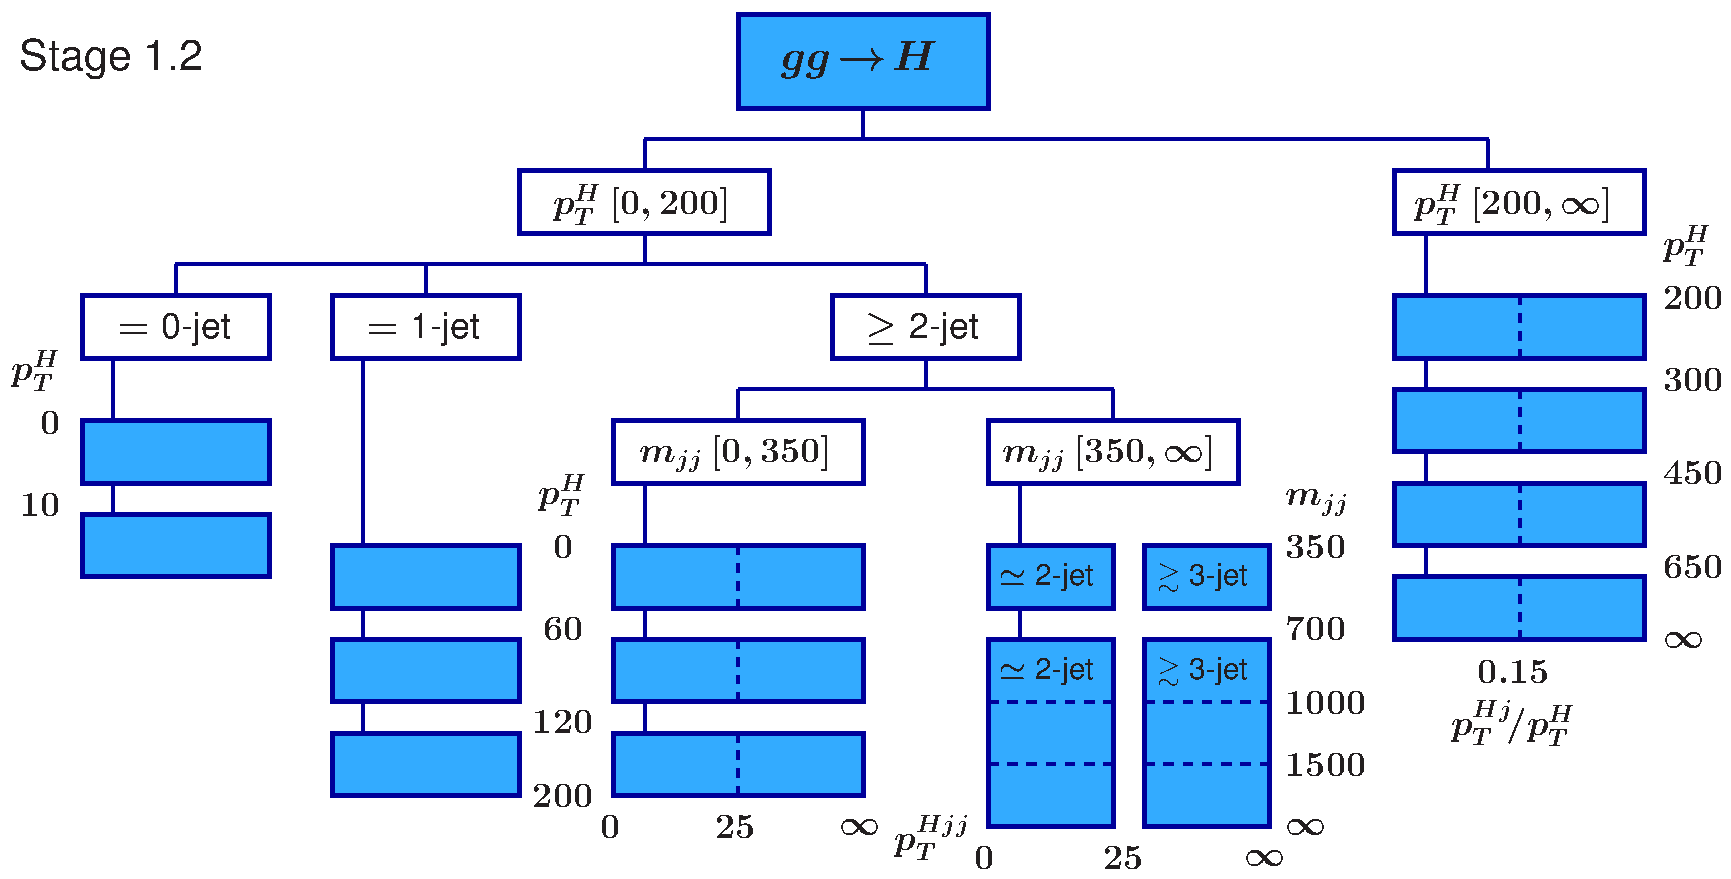
\includegraphics[width=0.8\textwidth]{figures/theory_chapter/simplifiedXS_ggF_1_2} \\[3mm]
  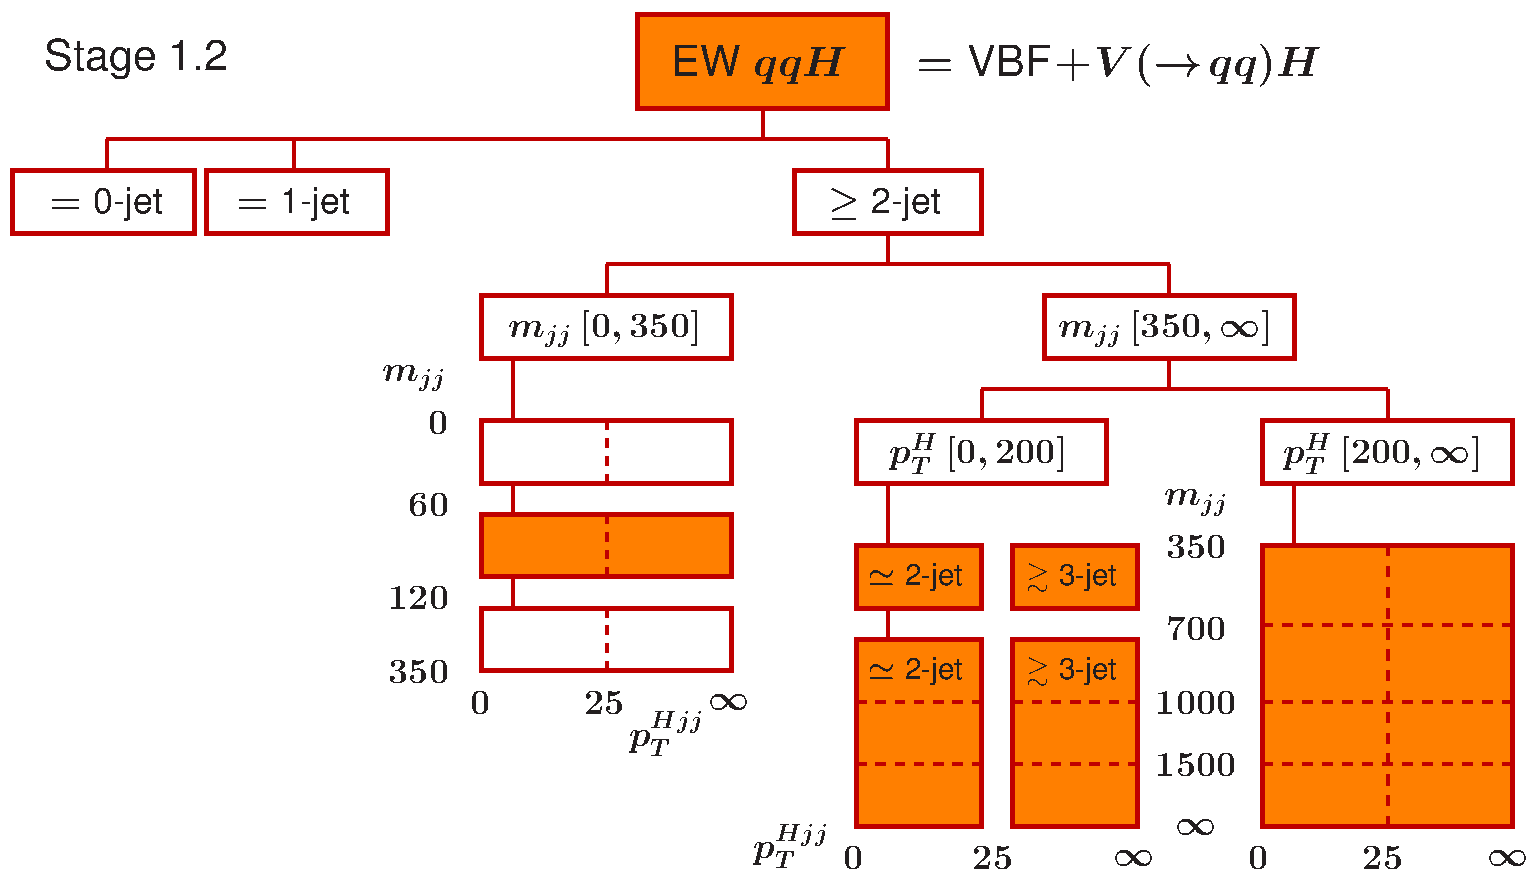
\includegraphics[width=0.8\textwidth]{figures/theory_chapter/simplifiedXS_VBF_1_2} \\[3mm]
  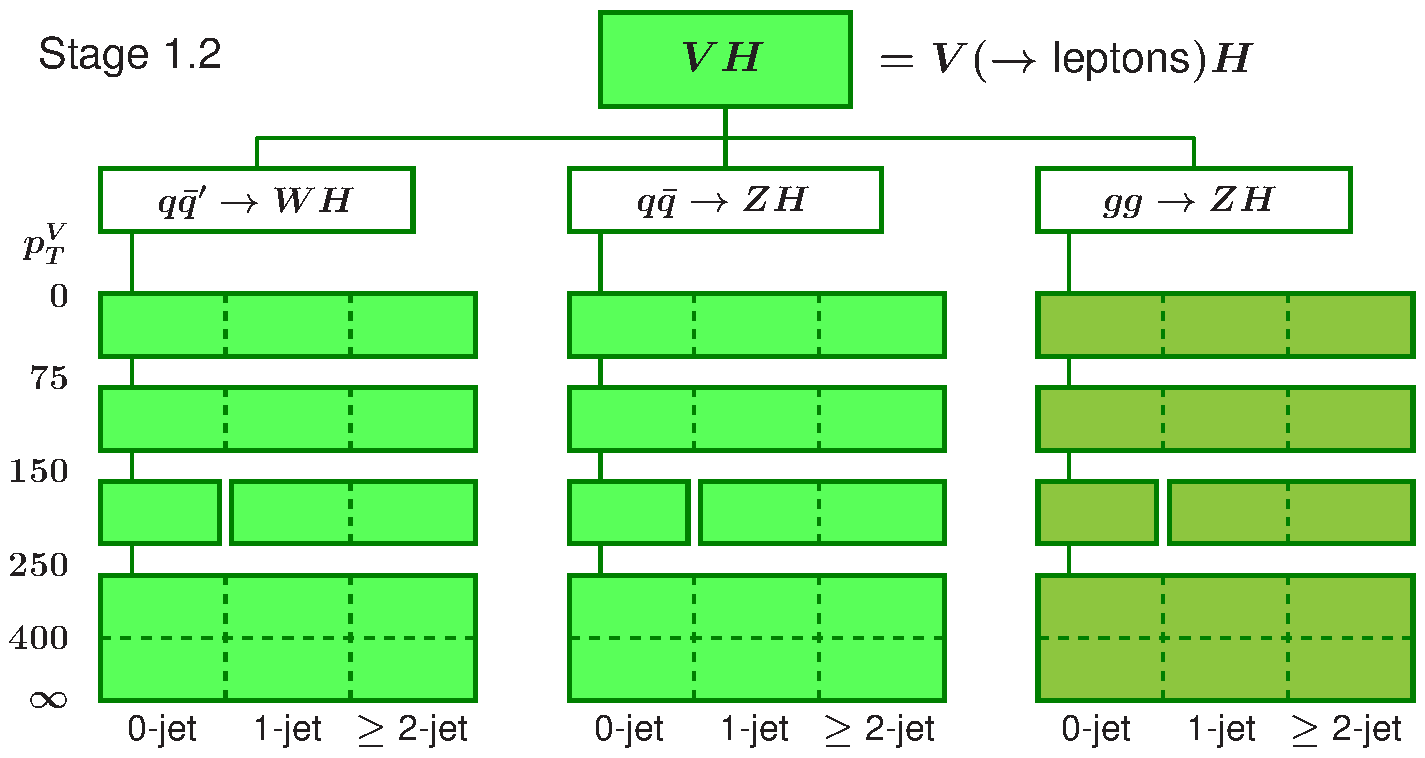
\includegraphics[width=0.6\textwidth]{figures/theory_chapter/simplifiedXS_VH_1_2}
  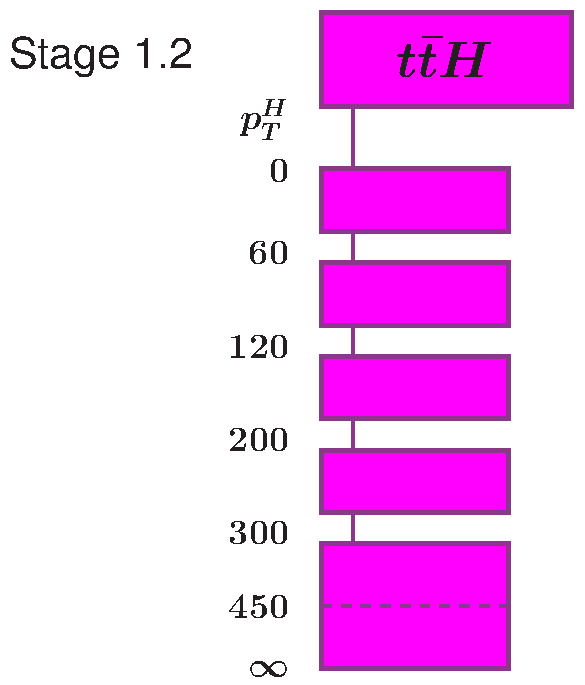
\includegraphics[width=0.25\textwidth]{figures/theory_chapter/simplifiedXS_ttH_1_2}
  \caption{Stage 1.2 STXS bin definitions for the main production modes.}
  \label{fig:STXS_scheme}
\end{figure}


In addition to their nominal production and decay modes, the $ggH$ STXS1.2 truth bins include both $ggF$ and hadronically-decaying $gg \rightarrow ZH$ events, while the $VBF$ STXS definition includes hadronically-decaying $qq \rightarrow VH$. Additionally, it is important to note that the leptonic $qq \rightarrow ZH$ and $gg \rightarrow ZH$ truth bins include Z-boson decays both to two charged leptons and to two neutrinos (the latter of which will have a high MET signature). For nomenclature purposes, throughout this dissertation, $ggF$ is used to refer to the $gg \rightarrow H$ production mode, while $ggH$ is used to refer to the regions of phase space targeting the combination of $gg \rightarrow H$ and $gg \rightarrow ZH$.

In the Couplings analysis, the experimental bins targeted are modified somewhat from the truth bins due to the inability to separate some processes: the $b\bar{b}H$ categories are subsumed into the $ggH$ categorization scheme, the leptonic $qq \rightarrow VH$ and $gg \rightarrow VH$ processes are combined into a series of $VHLep$ regions, $tH$ is split into $tWH$ and $tHjb$, and the $p_{T}^H > 200 GeV$ bin of the hadronic $qq \rightarrow VH$ truth category is split into two bins based on jet kinematics to aid in statistical combination with other analyses (where $p_{T}^{H}$ denotes the transverse momentum of the Higgs, that is, the component of the Higgs momentum perpendicular to the beamline). A total of 44 STXS truth regions are defined.

For all Monte Carlo simulated samples used to construct the STXS truth bins, the absolute value of the rapidity of the Higgs boson is required to satisfy $|y_{H}| < 2.5$ while jets, built with the anti-kT algorithm \cite{Cacciari_2008} using radius R=0.4, are required to have $p_{T} > 30 GeV$ (with the exception of the bins labelled FWDH, which target forward Higgs events with $|y_{H}| > 2.5$.

Using the Monte Carlo simulated samples described in section \ref{chap:DataMC}, we report the cross-section times branching ratio and acceptances (in terms of percentage of events of each production-mode) that fall into each STXS1.2 truth bin in Table \cite{STXS_cross_sections}, and show the acceptance for each production mode in Figure \ref{fig:STXS_acceptances}. Several of the STXS truth bins are merged in the Couplings analysis to account for effects such as the inability of the event classifier to discriminate between $qq \rightarrow ZH$ and $gg \rightarrow ZH$; this is detailed in section \ref{chap:CouplingsChapter}. By measuring the cross-sections in each of these bins, a number of different values are able to be extracted, including the various Higgs couplings $\kappa$ and limits on effective field theories (EFTs) parameterizing physics beyond the standard model.

\begin{table}[htbp]
        \centering
        {\footnotesize
        \begin{tabular}{lS}
                STXS 1.2 Truth Bin                                     & {$\sigma\times BR_{\gamma \gamma} [\si{\fb}]$} \\
                \hline
                gg2H\_0J\_ptH\_0\_10                                   & 15.038147                                    \\
                gg2H\_0J\_ptH\_gt10                                    & 46.799419                                    \\
                gg2H\_1J\_ptH\_0\_60                                   & 14.742653                                    \\
                gg2H\_1J\_ptH\_60\_120                                 & 10.223149                                    \\
                gg2H\_1J\_ptH\_120\_200                                & 1.692748                                     \\
                gg2H\_ge2J\_MJJ\_0\_350\_ptH\_0\_60                    & 2.639954                                     \\
                gg2H\_ge2J\_MJJ\_0\_350\_ptH\_60\_120                  & 4.058768                                     \\
                gg2H\_ge2J\_MJJ\_0\_350\_ptH\_120\_200                 & 2.133361                                     \\
                gg2H\_ge2J\_MJJ\_350\_700\_ptH\_0\_200\_ptHJJ\_0\_25   & 0.569488                                     \\
                gg2H\_ge2J\_MJJ\_350\_700\_ptH\_0\_200\_ptHJJ\_gt25    & 0.818394                                     \\
                gg2H\_ge2J\_MJJ\_gt700\_ptH\_0\_200\_ptHJJ\_0\_25      & 0.241653                                     \\
                gg2H\_ge2J\_MJJ\_gt700\_ptH\_0\_200\_ptHJJ\_gt25       & 0.363737                                     \\
                gg2H\_ptH\_200\_300                                    & 1.036991                                     \\
                gg2H\_ptH\_300\_450                                    & 0.239097                                     \\
                gg2H\_ptH\_450\_650                                    & 0.035624                                     \\
                gg2H\_ptH\_gt650                                       & 0.004947                                     \\
                qq2Hqq\_0J                                             & 0.816245                                     \\
                qq2Hqq\_1J                                             & 3.956656                                     \\
                qq2Hqq\_ge2J\_MJJ\_0\_60                               & 0.224649                                     \\
                qq2Hqq\_ge2J\_MJJ\_60\_120                             & 1.200933                                     \\
                qq2Hqq\_ge2J\_MJJ\_120\_350                            & 1.426903                                     \\
                qq2Hqq\_ge2J\_MJJ\_350\_700\_ptH\_0\_200\_ptHJJ\_0\_25 & 0.897833                                     \\
                qq2Hqq\_ge2J\_MJJ\_350\_700\_ptH\_0\_200\_ptHJJ\_gt25  & 0.337811                                     \\
                qq2Hqq\_ge2J\_MJJ\_gt700\_ptH\_0\_200\_ptHJJ\_0\_25    & 1.356668                                     \\
                qq2Hqq\_ge2J\_MJJ\_gt700\_ptH\_0\_200\_ptHJJ\_gt25     & 0.314044                                     \\
                qq2Hqq\_ge2J\_MJJ\_350\_700\_ptH\_gt200                & 0.104740                                     \\
                qq2Hqq\_ge2J\_MJJ\_gt700\_ptH\_gt200                   & 0.258838                                     \\
                qq2Hlnu\_ptV\_0\_75                                    & 0.466795                                     \\
                qq2Hlnu\_ptV\_75\_150                                  & 0.297442                                     \\
                qq2Hlnu\_ptV\_150\_250\_0J                             & 0.051545                                     \\
                qq2Hlnu\_ptV\_150\_250\_ge1J                           & 0.042651                                     \\
                qq2Hlnu\_ptV\_gt250                                    & 0.030152                                     \\
                qq2Hll\_ptV\_0\_75                                     & 0.236572                                     \\
                qq2Hll\_ptV\_75\_150                                   & 0.157167                                     \\
                qq2Hll\_ptV\_150\_250\_0J                              & 0.027476                                     \\
                qq2Hll\_ptV\_150\_250\_ge1J                            & 0.022523                                     \\
                qq2Hll\_ptV\_gt250                                     & 0.015076                                     \\
                gg2Hll\_ptV\_0\_75                                     & 0.014989                                     \\
                gg2Hll\_ptV\_75\_150                                   & 0.038219                                     \\
                gg2Hll\_ptV\_150\_250\_0J                              & 0.007812                                     \\
                gg2Hll\_ptV\_150\_250\_ge1J                            & 0.014855                                     \\
                gg2Hll\_ptV\_gt250                                     & 0.004465                                     \\
                ttH\_ptH\_0\_60                                        & 0.267960                                     \\
                ttH\_ptH\_60\_120                                      & 0.404152                                     \\
                ttH\_ptH\_120\_200                                     & 0.287483                                     \\
                ttH\_ptH\_200\_300                                     & 0.119454                                     \\
                ttH\_ptH\_gt300                                        & 0.055617                                     \\
                bbH                                                    & 1.044426                                     \\
                tH                                                     & 0.187064                                     \\
                \hline
        \end{tabular}
        }
        \caption{Simplified template cross sections times diphoton branching ratio for each of the STXS 1.2 truth bins.}
        \label{tab:STXS_cross_sections}
\end{table}

\begin{figure}[tbp]
        \centering
        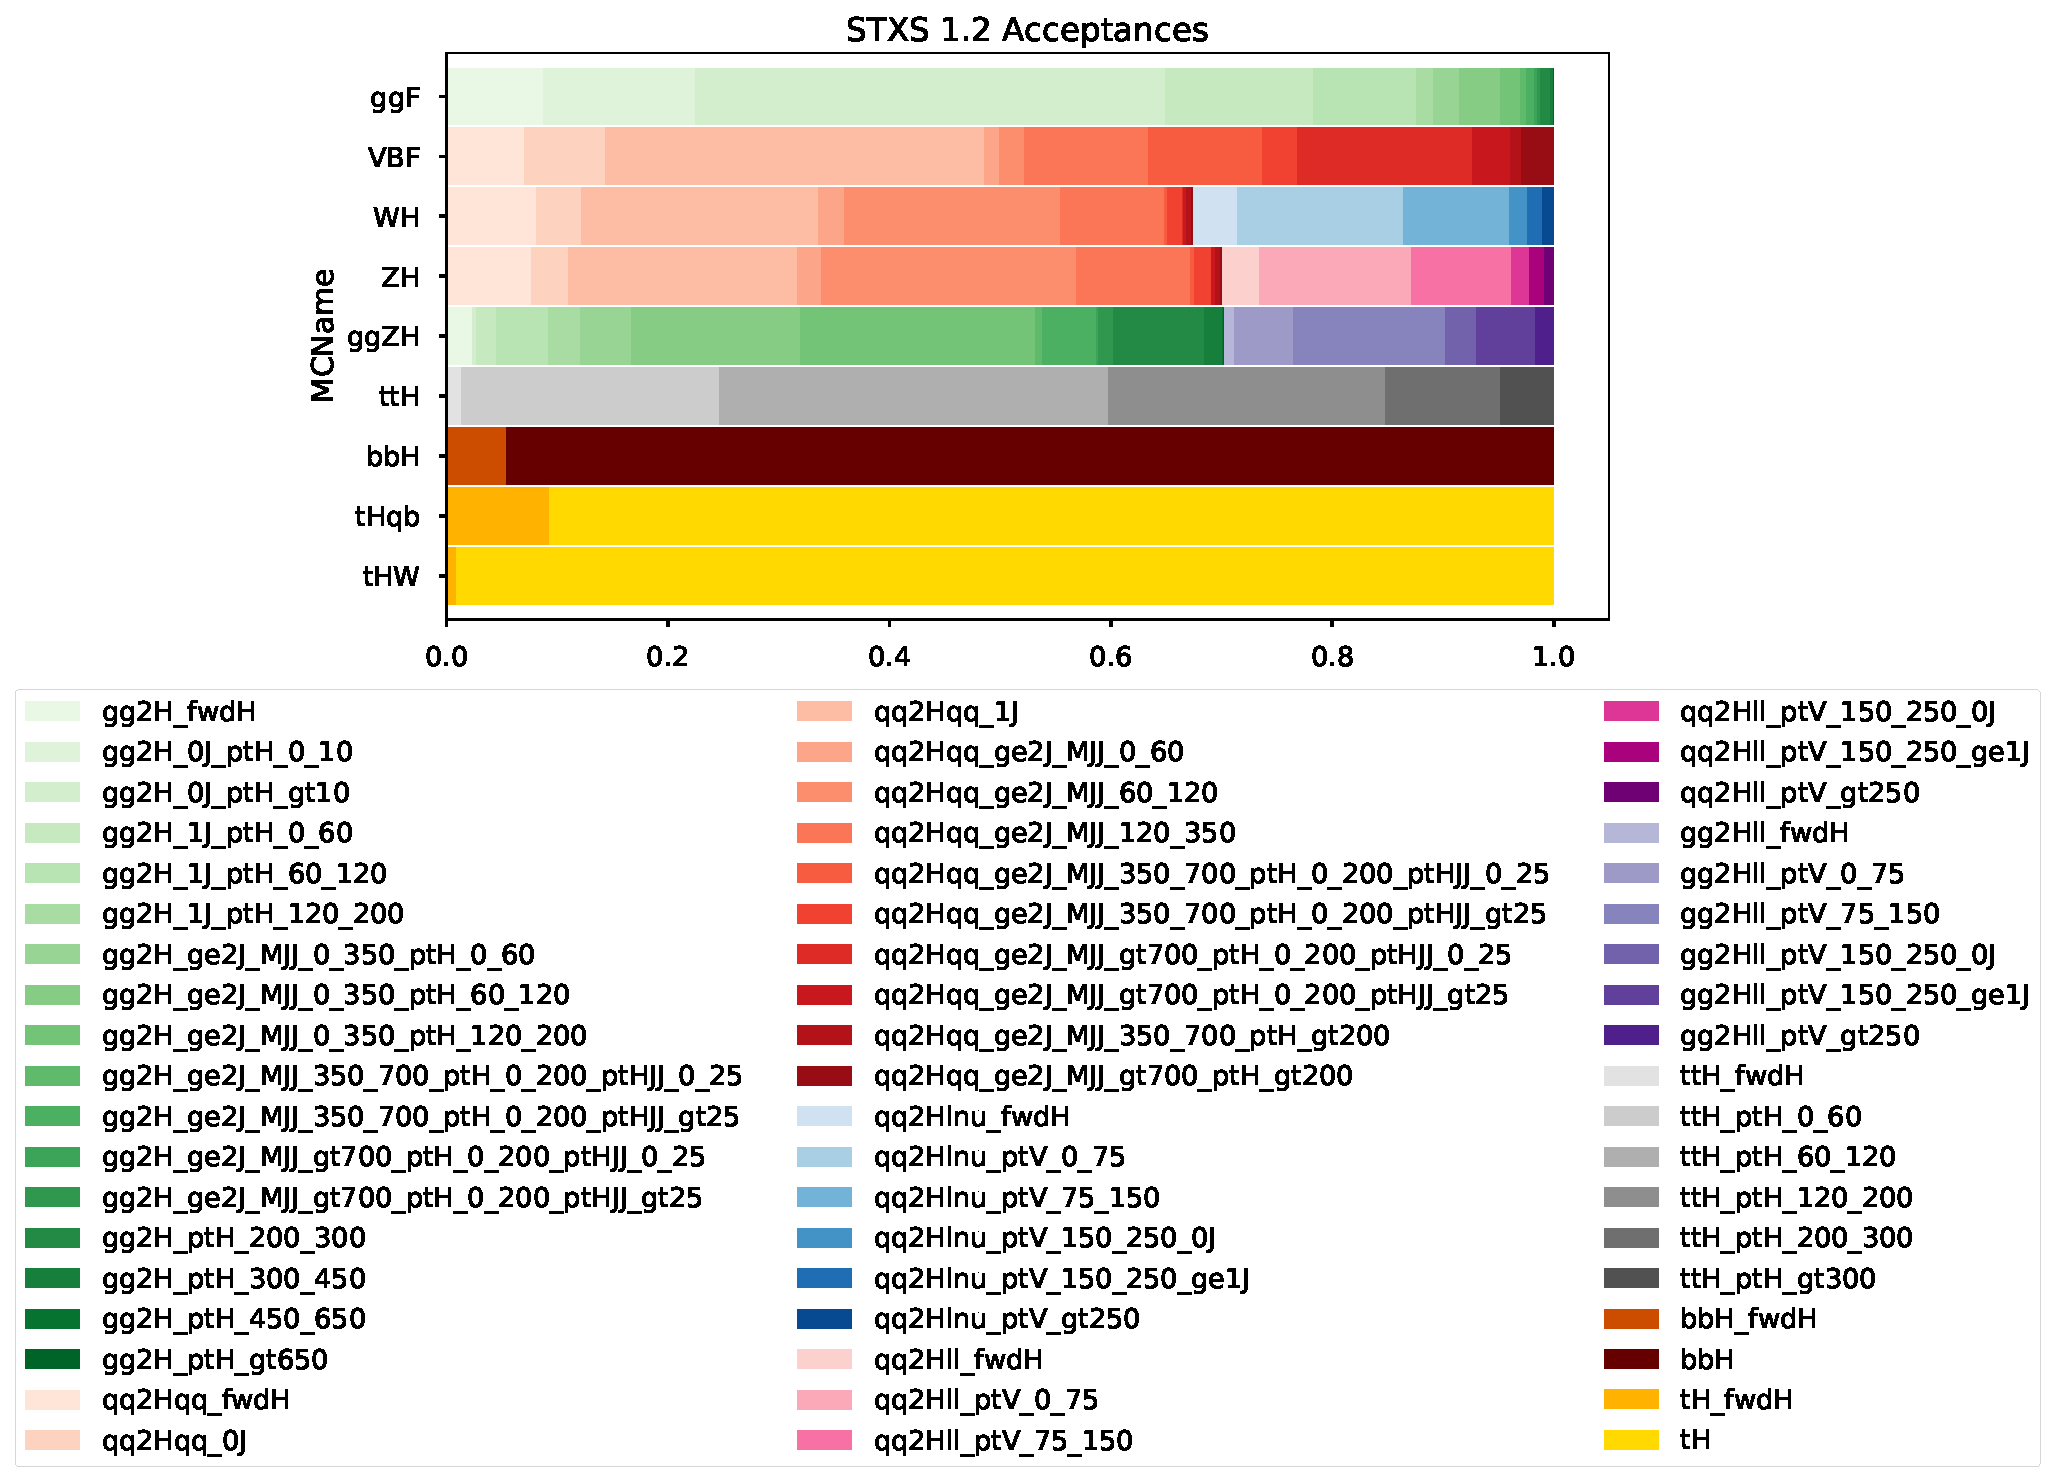
\includegraphics[width=\linewidth]{figures/theory_chapter/STXS_acceptances.pdf}
        \caption{Stage 1.2 STXS bin acceptances for all Higgs production modes considered in the Couplings analysis. The FWDH bins target events outside the nominal acceptance, i.e. with $|y_{H}|>2.5$.}
        \label{fig:STXS_acceptances}
\end{figure}


\iffalse
In addition to the kappa-framework, the Couplings Analysis also makes use of an Effective Field Theory (EFT) approach to parameterize potential Higgs Couplings beyond the Standard Model. Effective Field Theories offer a model-independent way to parameterize new physics that may not be directly accessible at LHC energies. Using the Standard Model Effective Field Theory parameterization (SMEFT) \cite{SMEFT}, we can write the Lagrangian for new physics that exists at some energy scale $\Lambda >> v$ (where $v$ denotes the Higgs field vacuum expectation value of 246 GeV) as

\begin{equation}
\mathcal{L}_{SMEFT} = \mathcal{L}_{SM} + (\frac{v}{\Lambda})\mathcal{L}_{5} + (\frac{v}{\Lambda})^2 \mathcal{L}_{6}
\end{equation}

If we assume that lepton and baryon number are conserved, we find that we cannot have any $\mathcal{L}_{5}$ operators, as all allowable dimension-5 operators violate the conservation of lepton number; thus, the leading EFT terms are all proportional to $(\frac{v}{\Lambda})^2$ and have dimension-6.

The dimension-6 Lagrangian term can be expanded as a linear combination of all allowable dimension-6 operators:

\begin{equation}
\mathcal{L}_{6} = \sum_{i} c_{i}^6 O_{i}^{6}
\end{equation}

In the Couplings Analysis, the operators are chosen using the so-called "Warsaw Basis" \cite{Warsaw}; the $c_{i}$ terms are the free parameters to be determined by the final likelihood fit, called "Wilson Coefficients". A list of all allowed dimension-6 operators and their corresponding coefficients is given in \ref{tab:EFT}.

\begin{table}
  \centering
  \begin{tabular}{c l}
  \hline
  Wilson coefficient & Operator \\
  \hline
  $\cHbox$ & $(H^\dag H)\Box(H^\dag H)$\\
  $\cHDD$   & $\ \left(H^\dag D^\mu H\right)^* \left(H^\dag D_\mu H\right)$\\
  $\cHG$  & $H^\dag H\, G^A_{\mu\nu} G^{A\mu\nu}$  \\
  $\cHB$ &  $ H^\dag H\, B_{\mu\nu} B^{\mu\nu}$\\
  $\cHW$ &  $H^\dag H\, W^I_{\mu\nu} W^{I\mu\nu}$\\
  $\cHWB$ &  $ H^\dag \tau^I H\, W^I_{\mu\nu} B^{\mu\nu}$\\
  $\cHl1$ & $(H^\dag i\overleftrightarrow{D}_\mu H)(\bar l_p \gamma^\mu l_r)$\\
  $\cHl3$ & $(H^\dag i\overleftrightarrow{D}^I_\mu H)(\bar l_p \tau^I \gamma^\mu l_r)$\\
  $\cHe$  & $(H^\dag i\overleftrightarrow{D}_\mu H)(\bar e_p \gamma^\mu e_r)$\\
  $\cHq1$ & $(H^\dag i\overleftrightarrow{D}_\mu H)(\bar q_p \gamma^\mu q_r)$\\
  $\cHq3$ & $(H^\dag i\overleftrightarrow{D}^I_\mu H)(\bar q_p \tau^I \gamma^\mu q_r)$\\
  $\cHu$  & $(H^\dag i\overleftrightarrow{D}_\mu H)(\bar u_p \gamma^\mu u_r)$\\
  $\cHd$  & $(H^\dag i\overleftrightarrow{D}_\mu H)(\bar d_p \gamma^\mu d_r)$\\
  $\cuGAbs$ & $(\bar q_p \sigma^{\mu\nu} T^A u_r) \widetilde H \, G_{\mu\nu}^A$ \\
  $\cll1$   & $(\bar l_p \gamma_\mu l_r)(\bar l_s \gamma^\mu l_t)$ \\
  \hline
\end{tabular}
  \caption{Wilson coefficients $c_i$ and corresponding dimension-6 SMEFT operators $\mathcal{O}_i$ used in this analysis.}
  \label{tab:EFT}
\end{table}

Under this model, we can write the cross-section in some STXS bin as 

\begin{equation}
\sigma_{bin} =  \sigma_{bin}^{SM} + \sigma_{bin}^{interaction} + \sigma_{bin}^{BSM}
\end{equation}

where the first term refers to the Standard-Model cross-section, the second refers to the interaction between the SM and BSM physics processes, and the last refers to the BSM processes themselves.

We can also write:
\begin{equation}
\frac{\sigma_{bin}^{interaction}}{\sigma_{bin}^{SM}} = \sum_{i} A_{i} c_{i}
\frac{\sigma_{bin}^{BSM}}{\sigma_{bin}^{SM}} = \sum_{i} B_{ij} c_{i} c_{j}
\end{equation}

So we can parameterize the cross-section as:
\begin{equation}
\frac{\sigma_{bin}}{\sigma_{bin}^{SM}} = 1 + \sum_{i} A_{i} c_{i} + \sum_{i} B_{ij} c_{i} c_{j}
\end{equation}

Similarly, the Higgs partial decay width to diphotons (a measure of how often the Higgs decays to diphotons vs other channels) can be parameterized as follows:

\begin{equation}
\Gamma_{\gamma \gamma} = \Gamma_{\gamma \gamma}^{SM} + \Gamma_{\gamma \gamma}^{interaction} + \Gamma_{\gamma \gamma}^{BSM}
\Gamma_{\gamma \gamma} = 1 + \sum_{i} A_{i}^{\Gamma_{\gamma \gamma}} c_{i} + \sum_{i} B_{ij}^{\Gamma_{\gamma \gamma}} c_{i} c_{j}
\end{equation}

Combining these, we can parameterize the event yield in each STXS bin in terms of the Wilson coefficients, using Monte Carlo simulated events to determine the $A_{i}$ and $B_{ij}$ coefficients. This is detailed further in Section \ref{sec:CouplingsChapter}.
\fi